\documentclass[12pt,a4paper]{article}
\usepackage[utf8]{inputenc}
\usepackage[spanish]{babel}
\usepackage{geometry}
\usepackage{graphicx}
\usepackage{fancyhdr}
\usepackage{titlesec}
\usepackage{enumitem}
\usepackage{url}
\usepackage{xcolor}
\usepackage{tcolorbox}
\usepackage{listings}
\usepackage{minted}
\usepackage{float}

% Configuración de página
\geometry{margin=2.5cm}
\pagestyle{fancy}
\fancyhf{}
\fancyhead[L]{Informe Técnico de Auditoría - CEMSE}
\fancyhead[R]{\thepage}
\renewcommand{\headrulewidth}{0.4pt}

% Configuración de títulos
\titleformat{\section}{\Large\bfseries\color{blue!70!black}}{\thesection}{1em}{}
\titleformat{\subsection}{\large\bfseries\color{blue!50!black}}{\thesubsection}{1em}{}

% Configuración de código
\lstset{
    basicstyle=\ttfamily\footnotesize,
    breaklines=true,
    frame=single,
    numbers=left,
    numberstyle=\tiny,
    backgroundcolor=\color{gray!10}
}

\begin{document}

% 0. Portada
\begin{titlepage}
    \centering
    \vspace*{2cm}

    {\Huge\bfseries INFORME TÉCNICO DE AUDITORÍA\\[0.5cm]}
    {\LARGE Plataforma Educativa CEMSE\\[2cm]}

    \begin{tcolorbox}[colback=red!5!white,colframe=red!75!black,width=0.8\textwidth]
        \centering
        \large
        \textbf{Análisis Integral del Repositorio}\\
        Sistema de Gestión Educativa, Empleo y Emprendimiento
    \end{tcolorbox}

    \vfill

    {\large \textbf{Repositorio:} C:\textbackslash Users\textbackslash david\textbackslash projects\textbackslash asd\textbackslash cemse\\[0.3cm]}
    {\large \textbf{Rama:} master\\[0.3cm]}
    {\large \textbf{Commit:} 535dba0\\[0.3cm]}
    {\large \textbf{Fecha de Auditoría:} \today}

\end{titlepage}

\newpage
\tableofcontents
\newpage

% 1. Resumen
\section{Resumen}

CEMSE es una plataforma web integral para gestión educativa desarrollada con Next.js 15, que integra funcionalidades de cursos, empleo juvenil, emprendimiento e instituciones educativas. El sistema maneja múltiples roles de usuario y proporciona herramientas especializadas para cada tipo de actor en el ecosistema educativo-laboral.

\textbf{Tecnologías principales identificadas:}
\begin{itemize}
    \item \textbf{Frontend:} Next.js 15.1.7 con React 19 y TypeScript 5
    \item \textbf{Base de Datos:} PostgreSQL con Prisma ORM 6.16.1
    \item \textbf{Autenticación:} NextAuth.js 4.24.11
    \item \textbf{Almacenamiento:} MinIO 8.0.6 para objetos
    \item \textbf{UI:} Tailwind CSS con componentes Radix UI
    \item \textbf{Testing:} Jest 30.1.3 con Testing Library
\end{itemize}

% 2. Inventario
\section{Inventario}

\subsection{Árbol de carpetas principales}

\begin{verbatim}
cemse/
├── src/                    # Código fuente principal
│   ├── app/               # Next.js App Router
│   │   ├── (auth)/       # Rutas de autenticación
│   │   ├── (dashboard)/  # Panel principal
│   │   └── api/          # Endpoints de API
│   ├── components/        # Componentes React
│   ├── hooks/            # Hooks personalizados
│   ├── lib/              # Utilidades y servicios
│   └── types/            # Definiciones TypeScript
├── prisma/                # Esquemas de base de datos
├── scripts/               # Scripts de utilidad
├── tasks/                 # Documentación y tareas
├── public/                # Archivos estáticos
├── __tests__/             # Tests unitarios
└── docs/                  # Documentación adicional
\end{verbatim}

\subsection{Archivos clave identificados}

\textbf{Manifiestos:}
\begin{itemize}
    \item \texttt{package.json} - Dependencias y scripts de Node.js
    \item \texttt{pnpm-lock.yaml} - Lockfile del gestor de paquetes
    \item \texttt{pnpm-workspace.yaml} - Configuración de workspace
\end{itemize}

\textbf{Documentación:}
\begin{itemize}
    \item \texttt{README.md} - Documentación principal del proyecto
    \item \texttt{DEPLOYMENT.md} - Guía de despliegue
    \item \texttt{cemse.md} - Documentación extendida del sistema
\end{itemize}

\textbf{CI/CD:}
\begin{itemize}
    \item No encontrado - No se detectaron archivos \texttt{.github/workflows} en el directorio raíz
\end{itemize}

\textbf{Infraestructura:}
\begin{itemize}
    \item \texttt{Dockerfile} - Configuración de contenedor
    \item \texttt{docker-compose.yml} - Orquestación de servicios
    \item \texttt{manage.sh} - Script de gestión del sistema
    \item \texttt{setup.sh} - Script de configuración inicial
    \item \texttt{setup-ubuntu.sh} - Script específico para Ubuntu
\end{itemize}

\textbf{Configuración:}
\begin{itemize}
    \item \texttt{env.template} - Plantilla de variables de entorno
    \item \texttt{next.config.ts} - Configuración de Next.js
    \item \texttt{tsconfig.json} - Configuración de TypeScript
    \item \texttt{tailwind.config.ts} - Configuración de Tailwind CSS
    \item \texttt{eslint.config.mjs} - Configuración de ESLint
    \item \texttt{jest.config.js} - Configuración de Jest
\end{itemize}

\textbf{Tests:}
\begin{itemize}
    \item \texttt{\_\_tests\_\_/} - Directorio de tests unitarios
    \item \texttt{jest.setup.js} - Configuración inicial de Jest
\end{itemize}

\textbf{API/Esquemas:}
\begin{itemize}
    \item \texttt{prisma/schema.prisma} - Esquema de base de datos
    \item No encontrado - No se detectaron archivos OpenAPI/Swagger
    \item No encontrado - No se detectaron archivos gRPC/Protocol Buffers
\end{itemize}

% 3. Stack y versiones
\section{Stack y versiones}

\subsection{Dependencias principales (desde package.json)}

\textbf{Runtime y Framework:}
\begin{itemize}
    \item \texttt{next@15.1.7} - Framework React para producción
    \item \texttt{react@19.0.0} - Biblioteca de UI
    \item \texttt{react-dom@19.0.0} - DOM bindings para React
    \item \texttt{typescript@5} - Superset tipado de JavaScript
\end{itemize}

\textbf{Base de Datos:}
\begin{itemize}
    \item \texttt{@prisma/client@6.16.1} - Cliente ORM
    \item \texttt{prisma@6.16.1} - Herramientas de base de datos
\end{itemize}

\textbf{Autenticación:}
\begin{itemize}
    \item \texttt{next-auth@4.24.11} - Autenticación para Next.js
    \item \texttt{@auth/prisma-adapter@2.10.0} - Adaptador para Prisma
    \item \texttt{bcryptjs@3.0.2} - Hashing de contraseñas
\end{itemize}

\textbf{UI y Estilos:}
\begin{itemize}
    \item \texttt{tailwindcss@3.4.1} - Framework CSS utility-first
    \item \texttt{@radix-ui/*} - Componentes UI primitivos (v1.x-v2.x)
    \item \texttt{framer-motion@12.23.12} - Animaciones
    \item \texttt{lucide-react@0.544.0} - Iconos
\end{itemize}

\textbf{Almacenamiento y Archivos:}
\begin{itemize}
    \item \texttt{minio@8.0.6} - Cliente para almacenamiento de objetos
    \item \texttt{@react-pdf/renderer@4.3.0} - Generación de PDFs
    \item \texttt{canvas@3.2.0} - Renderizado de canvas
\end{itemize}

\textbf{Utilidades:}
\begin{itemize}
    \item \texttt{@tanstack/react-query@5.87.4} - Gestión de estado server
    \item \texttt{react-hook-form@7.62.0} - Gestión de formularios
    \item \texttt{zod@4.1.8} - Validación de esquemas
    \item \texttt{date-fns@4.1.0} - Manipulación de fechas
    \item \texttt{crypto-js@4.2.0} - Utilidades criptográficas
\end{itemize}

\textbf{Mapas y Geolocalización:}
\begin{itemize}
    \item \texttt{leaflet@1.9.4} - Biblioteca de mapas
    \item \texttt{react-leaflet@5.0.0} - Integración React-Leaflet
\end{itemize}

\subsection{Dependencias de desarrollo}

\textbf{Testing:}
\begin{itemize}
    \item \texttt{jest@30.1.3} - Framework de testing
    \item \texttt{@testing-library/react@16.3.0} - Testing utilities
    \item \texttt{@testing-library/jest-dom@6.8.0} - Matchers Jest DOM
\end{itemize}

\textbf{Linting y Calidad:}
\begin{itemize}
    \item \texttt{eslint@9} - Linter JavaScript/TypeScript
    \item \texttt{prettier@3.6.2} - Formateador de código
    \item \texttt{eslint-config-next@15.1.7} - Configuración ESLint para Next.js
\end{itemize}

% 4. Arquitectura
\section{Arquitectura}

\subsection{Patrón arquitectónico}

El proyecto implementa una \textbf{arquitectura modular basada en Next.js App Router} con separación clara de responsabilidades:

\begin{itemize}
    \item \textbf{Capa de Presentación:} Componentes React con Tailwind CSS
    \item \textbf{Capa de Lógica de Negocio:} API Routes de Next.js
    \item \textbf{Capa de Datos:} Prisma ORM con PostgreSQL
    \item \textbf{Capa de Almacenamiento:} MinIO para archivos multimedia
    \item \textbf{Capa de Autenticación:} NextAuth.js con adaptador Prisma
\end{itemize}

\subsection{Límites de contexto identificados}

\begin{enumerate}
    \item \textbf{Contexto de Autenticación} (\texttt{src/app/(auth)/})
    \item \textbf{Contexto de Dashboard} (\texttt{src/app/(dashboard)/})
    \item \textbf{Contexto de API} (\texttt{src/app/api/})
    \item \textbf{Contexto de Cursos} (\texttt{src/components/courses/})
    \item \textbf{Contexto de Empleos} (\texttt{src/components/jobs/})
    \item \textbf{Contexto de Emprendimiento} (\texttt{src/components/entrepreneurship/})
    \item \textbf{Contexto de Instituciones} (\texttt{src/components/institutions/})
    \item \textbf{Contexto de Empresas} (\texttt{src/components/companies/})
\end{enumerate}

% 5. Módulos/Servicios
\section{Módulos/Servicios}

\subsection{Módulos principales identificados}

\textbf{Sistema de Autenticación:}
\begin{itemize}
    \item \texttt{src/app/api/auth/} - Endpoints de autenticación
    \item \texttt{src/app/(auth)/} - Páginas de login/registro
    \item Roles: YOUTH, COMPANIES, INSTITUTION, SUPERADMIN
\end{itemize}

\textbf{Gestión de Cursos:}
\begin{itemize}
    \item \texttt{src/components/courses/} - Componentes de cursos
    \item \texttt{src/app/api/courses/} - API de cursos
    \item Funcionalidades: enrollments, certificates, quizzes, progress
\end{itemize}

\textbf{Portal de Empleo:}
\begin{itemize}
    \item \texttt{src/components/jobs/} - Componentes de empleos
    \item \texttt{src/app/api/jobs/} - API de ofertas laborales
    \item Funcionalidades: applications, filters, status tracking
\end{itemize}

\textbf{Emprendimiento:}
\begin{itemize}
    \item \texttt{src/components/entrepreneurship/} - Red social emprendedores
    \item \texttt{src/app/api/entrepreneurship/} - API de emprendimiento
    \item Funcionalidades: posts, connections, resources, calculator
\end{itemize}

\textbf{Gestión de Archivos:}
\begin{itemize}
    \item \texttt{src/app/api/files/} - API de archivos
    \item \texttt{src/components/files/} - Gestión de archivos
    \item Integración con MinIO para almacenamiento
\end{itemize}

\textbf{Analíticas:}
\begin{itemize}
    \item \texttt{src/components/analytics/} - Dashboards y métricas
    \item \texttt{src/app/api/analytics/} - API de analíticas
    \item Reportes por módulo y usuario
\end{itemize}

% 6. API
\section{API}

\subsection{Endpoints principales identificados}

\textbf{Autenticación:}
\begin{itemize}
    \item \texttt{POST /api/auth/[...nextauth]} - NextAuth.js endpoints
    \item \texttt{POST /api/auth/register} - Registro de usuarios
    \item \texttt{POST /api/auth/forgot-password} - Recuperación de contraseñas
    \item \texttt{POST /api/auth/reset-password} - Reset de contraseñas
\end{itemize}

\textbf{Cursos:}
\begin{itemize}
    \item \texttt{GET/POST /api/courses} - CRUD de cursos
    \item \texttt{POST /api/courses/[id]/enroll} - Inscripción a cursos
    \item \texttt{GET /api/courses/[id]/modules} - Módulos de curso
    \item \texttt{GET /api/courses/categories} - Categorías disponibles
    \item \texttt{GET /api/courses/analytics} - Analíticas de cursos
\end{itemize}

\textbf{Empleos:}
\begin{itemize}
    \item \texttt{GET/POST /api/jobs} - Ofertas laborales
    \item \texttt{GET /api/jobs/[id]} - Detalle de oferta
    \item \texttt{POST /api/jobs/[id]/apply} - Aplicar a empleo
    \item \texttt{GET /api/companies/[id]/jobs} - Empleos por empresa
\end{itemize}

\textbf{Archivos:}
\begin{itemize}
    \item \texttt{POST /api/files/upload} - Subida de archivos
    \item \texttt{POST /api/files/chunked-upload} - Subida por chunks
    \item \texttt{GET /api/files/minio/presigned} - URLs firmadas MinIO
    \item \texttt{GET /api/files/minio/status} - Estado del servidor MinIO
\end{itemize}

\textbf{Mensajería:}
\begin{itemize}
    \item \texttt{GET/POST /api/messages} - Sistema de mensajes
    \item \texttt{GET /api/messages/conversations} - Conversaciones
    \item Contextos: JOB\_APPLICATION, ENTREPRENEURSHIP, GENERAL
\end{itemize}

\subsection{Esquemas de autenticación}

\textbf{NextAuth.js implementado:}
\begin{itemize}
    \item Estrategia: Credentials Provider
    \item Sesiones: JWT con Prisma adapter
    \item Roles: Control de acceso basado en UserRole enum
\end{itemize}

% 7. Datos
\section{Datos}

\subsection{Base de datos PostgreSQL}

\textbf{Archivo de esquema:} \texttt{prisma/schema.prisma}

\textbf{Entidades principales identificadas:}

\begin{enumerate}
    \item \textbf{User} - Usuarios del sistema (4 roles)
    \item \textbf{Profile} - Perfiles extendidos de usuarios
    \item \textbf{Course} - Cursos educativos
    \item \textbf{CourseModule} - Módulos de cursos
    \item \textbf{Lesson} - Lecciones individuales
    \item \textbf{JobOffer} - Ofertas laborales
    \item \textbf{JobApplication} - Aplicaciones a empleos
    \item \textbf{YouthApplication} - Aplicaciones abiertas de jóvenes
    \item \textbf{Company} - Empresas empleadoras
    \item \textbf{Institution} - Instituciones educativas
    \item \textbf{Entrepreneurship} - Emprendimientos
    \item \textbf{NewsArticle} - Artículos de noticias
    \item \textbf{Resource} - Recursos educativos
    \item \textbf{Message} - Sistema de mensajería
    \item \textbf{BusinessPlan} - Planes de negocio
\end{itemize}

\textbf{Enums definidos:}
\begin{itemize}
    \item UserRole, UserStatus, InstitutionType
    \item EducationLevel, ExperienceLevel, CompanySize
    \item JobStatus, ApplicationStatus, ContractType, WorkModality
    \item CourseCategory, CourseLevel, LessonType
    \item BusinessStage, NewsType, NewsStatus, PostType
\end{itemize}

\textbf{Relaciones complejas identificadas:}
\begin{itemize}
    \item User 1:1 Profile (con cascade delete)
    \item Course 1:N CourseModule 1:N Lesson
    \item JobOffer 1:N JobApplication N:1 Profile
    \item Company 1:N JobOffer, Company N:1 Institution
    \item Mensaje con contexto (MessageContextType)
    \item Conexiones de emprendimiento (PENDING/ACCEPTED/DECLINED)
\end{itemize}

\subsection{Migraciones y seeds}

\textbf{Migraciones:} Manejadas por Prisma (comando \texttt{prisma migrate})
\textbf{Seeds disponibles:}
\begin{itemize}
    \item \texttt{prisma/seed.ts} - Seed básico
    \item \texttt{prisma/seed-enhanced.ts} - Seed extendido
\end{itemize}

% 8. Infra/DevOps
\section{Infra/DevOps}

\subsection{Contenedorización}

\textbf{Docker configurado:}
\begin{itemize}
    \item \texttt{Dockerfile} - Imagen de la aplicación Next.js
    \item \texttt{docker-compose.yml} - Orquestación multi-servicio
\end{itemize}

\textbf{Servicios en docker-compose:}
\begin{itemize}
    \item \texttt{postgres} - Base de datos PostgreSQL
    \item \texttt{redis} - Cache y sesiones
    \item \texttt{minio} - Almacenamiento de objetos
    \item \texttt{prisma-studio} - UI de administración DB (desarrollo)
\end{itemize}

\subsection{Scripts de gestión}

\textbf{Scripts de setup:}
\begin{itemize}
    \item \texttt{setup.sh} - Configuración inicial general
    \item \texttt{setup-ubuntu.sh} - Configuración específica Ubuntu
    \item \texttt{manage.sh} - Gestión del sistema (start/stop/deploy)
    \item \texttt{update.sh} - Actualización del sistema
\end{itemize}

\textbf{Scripts de utilidad:}
\begin{itemize}
    \item \texttt{scripts/init-minio.js} - Inicialización MinIO
    \item \texttt{scripts/test-image-proxy.js} - Test de proxy de imágenes
    \item \texttt{scripts/migrate-course-thumbnails.js} - Migración thumbnails
\end{itemize}

\subsection{Variables de entorno}

\textbf{Archivo template:} \texttt{env.template}
\textbf{Variables principales (nombres):}
\begin{itemize}
    \item \texttt{DATABASE\_URL} - Conexión PostgreSQL
    \item \texttt{NEXTAUTH\_SECRET} - Secreto para autenticación
    \item \texttt{MINIO\_*} - Configuración MinIO
    \item \texttt{REDIS\_URL} - Conexión Redis
    \item \texttt{NODE\_ENV} - Entorno de ejecución
\end{itemize}

% 9. Observabilidad/Calidad/Seguridad
\section{Observabilidad/Calidad/Seguridad}

\subsection{Testing}

\textbf{Framework de testing:} Jest 30.1.3
\textbf{Archivos de configuración:}
\begin{itemize}
    \item \texttt{jest.config.js} - Configuración principal
    \item \texttt{jest.setup.js} - Setup inicial
\end{itemize}
\textbf{Scripts de testing:}
\begin{itemize}
    \item \texttt{npm run test} - Ejecutar tests
    \item \texttt{npm run test:watch} - Tests en modo watch
    \item \texttt{npm run test:coverage} - Cobertura de código
\end{itemize}

\subsection{Linting y calidad}

\textbf{ESLint configurado:}
\begin{itemize}
    \item \texttt{eslint.config.mjs} - Configuración ESLint 9
    \item \texttt{npm run lint} - Análisis de código
\end{itemize}

\textbf{Prettier integrado:}
\begin{itemize}
    \item \texttt{prettier@3.6.2} - Formateador automático
    \item \texttt{eslint-plugin-prettier} - Integración ESLint-Prettier
\end{itemize}

\subsection{Seguridad}

\textbf{Autenticación y autorización:}
\begin{itemize}
    \item NextAuth.js con JWT
    \item Hashing con bcryptjs
    \item Control de acceso basado en roles
\end{itemize}

\textbf{Configuración de seguridad en Next.js:}
\begin{itemize}
    \item Headers de seguridad (CSP, X-Frame-Options, etc.)
    \item Configuración CORS en \texttt{next.config.ts}
    \item Validación con Zod
\end{itemize}

\textbf{Dependencias sensibles identificadas:}
\begin{itemize}
    \item \texttt{crypto-js} - Operaciones criptográficas
    \item \texttt{bcryptjs} - Hashing de contraseñas
    \item MinIO para almacenamiento seguro
\end{itemize}

% 10. Documentación
\section{Documentación}

\textbf{Documentación encontrada:}
\begin{itemize}
    \item \texttt{README.md} - Documentación principal con instrucciones de setup
    \item \texttt{DEPLOYMENT.md} - Guía detallada de despliegue
    \item \texttt{cemse.md} - Documentación extendida del sistema
    \item \texttt{tasks/} - Documentación de tareas y informes
\end{itemize}

\textbf{Documentación de API:} No encontrado - No se detectaron archivos OpenAPI/Swagger

\textbf{Documentación de código:} Comentarios inline en TypeScript

% 11. UX/UI — Esquema con subniveles
\section{UX/UI — Esquema con subniveles}

\subsection{Lista jerárquica de vistas}

\textbf{Autenticación:}
\begin{itemize}
    \item Sign In (\texttt{src/app/(auth)/sign-in/page.tsx})
    \item Sign Up (\texttt{src/app/(auth)/sign-up/page.tsx})
    \item Forgot Password (\texttt{src/app/(auth)/forgot-password/page.tsx})
    \item Reset Password (\texttt{src/app/(auth)/reset-password/page.tsx})
\end{itemize}

\textbf{Dashboard Principal:}
\begin{itemize}
    \item Dashboard Home (\texttt{src/app/(dashboard)/page.tsx})
    \item Analytics (\texttt{src/app/(dashboard)/analytics/page.tsx})
    \item Search (\texttt{src/app/(dashboard)/search/page.tsx})
    \item Settings (\texttt{src/app/(dashboard)/settings/page.tsx})
    \item Messages (\texttt{src/app/(dashboard)/messages/page.tsx})
\end{itemize}

\textbf{Cursos:}
\begin{itemize}
    \item Courses List (\texttt{src/app/(dashboard)/courses/page.tsx})
    \item Course Detail (\texttt{src/app/(dashboard)/courses/[id]/page.tsx})
    \item Course Edit (\texttt{src/app/(dashboard)/courses/[id]/edit/page.tsx})
    \item Certificates (\texttt{src/app/(dashboard)/certificates/page.tsx})
    \item Quizzes (\texttt{src/app/(dashboard)/quizzes/page.tsx})
    \item Discussions (\texttt{src/app/(dashboard)/discussions/page.tsx})
\end{itemize}

\textbf{Empleos:}
\begin{itemize}
    \item Jobs List (\texttt{src/app/(dashboard)/jobs/page.tsx})
    \item Job Detail (\texttt{src/app/(dashboard)/jobs/[id]/page.tsx})
    \item Job Apply (\texttt{src/app/(dashboard)/jobs/[id]/apply/page.tsx})
    \item Job Edit (\texttt{src/app/(dashboard)/jobs/[id]/edit/page.tsx})
    \item Job Analytics (\texttt{src/app/(dashboard)/jobs/[id]/analytics/page.tsx})
    \item Job Chat (\texttt{src/app/(dashboard)/jobs/[id]/chat/page.tsx})
    \item Bookmarked Jobs (\texttt{src/app/(dashboard)/jobs/bookmarked/page.tsx})
    \item Saved Searches (\texttt{src/app/(dashboard)/jobs/saved-searches/page.tsx})
    \item Job Applications (\texttt{src/app/(dashboard)/jobs/[id]/applications/page.tsx})
\end{itemize}

\textbf{Emprendimiento:}
\begin{itemize}
    \item Entrepreneurship Home (\texttt{src/app/(dashboard)/entrepreneurship/page.tsx})
    \item Network (\texttt{src/app/(dashboard)/entrepreneurship/network/page.tsx})
    \item Connections (\texttt{src/app/(dashboard)/entrepreneurship/connections/page.tsx})
    \item Calculator (\texttt{src/app/(dashboard)/entrepreneurship/calculator/page.tsx})
    \item Analytics (\texttt{src/app/(dashboard)/entrepreneurship/analytics/page.tsx})
\end{itemize}

\textbf{Perfiles:}
\begin{itemize}
    \item My Profile (\texttt{src/app/(dashboard)/profile/page.tsx})
    \item Profile Files (\texttt{src/app/(dashboard)/profile/files/page.tsx})
    \item CV Builder (\texttt{src/app/(dashboard)/cv-builder/page.tsx})
    \item Profiles List (\texttt{src/app/(dashboard)/profiles/page.tsx})
    \item Profile Detail (\texttt{src/app/(dashboard)/profiles/[id]/page.tsx})
\end{itemize}

\textbf{Administración:}
\begin{itemize}
    \item Admin Dashboard (\texttt{src/app/(dashboard)/admin/page.tsx})
    \item Admin Users (\texttt{src/app/(dashboard)/admin/users/page.tsx})
    \item Admin Companies (\texttt{src/app/(dashboard)/admin/companies/page.tsx})
    \item Admin Institutions (\texttt{src/app/(dashboard)/admin/institutions/page.tsx})
\end{itemize}

\subsection{Diagrama Mermaid de flujo de navegación}

\begin{minted}{mermaid}
graph TD
    A[Sign In] --> B[Dashboard]
    B --> C[Courses]
    B --> D[Jobs]
    B --> E[Entrepreneurship]
    B --> F[Profile]
    B --> G[Admin Panel]

    C --> C1[Course List]
    C --> C2[My Certificates]
    C --> C3[Quizzes]
    C1 --> C4[Course Detail]
    C4 --> C5[Lessons & Modules]

    D --> D1[Job Search]
    D --> D2[My Applications]
    D --> D3[Bookmarked Jobs]
    D1 --> D4[Job Detail]
    D4 --> D5[Apply to Job]
    D4 --> D6[Job Chat]

    E --> E1[Network]
    E --> E2[My Connections]
    E --> E3[Business Calculator]
    E --> E4[Analytics]

    F --> F1[Edit Profile]
    F --> F2[CV Builder]
    F --> F3[Files Manager]

    G --> G1[Manage Users]
    G --> G2[Manage Companies]
    G --> G3[Manage Institutions]
    G --> G4[System Analytics]
\end{minted}

% 12. Ejecución/Despliegue
\section{Ejecución/Despliegue}

\subsection{Desarrollo local}

\textbf{Comandos principales:}
\begin{verbatim}
# Instalación
pnpm install

# Configuración
cp env.template .env

# Infraestructura
pnpm run docker:up

# Desarrollo
pnpm run dev
\end{verbatim}

\textbf{Puntos de acceso desarrollo:}
\begin{itemize}
    \item \textbf{Aplicación:} http://localhost:3000
    \item \textbf{MinIO Console:} http://localhost:9001
    \item \textbf{Prisma Studio:} http://localhost:5555
\end{itemize}

\subsection{Scripts de gestión disponibles}

\textbf{Ciclo de vida:}
\begin{itemize}
    \item \texttt{./manage.sh start} - Iniciar servicios
    \item \texttt{./manage.sh stop} - Detener servicios
    \item \texttt{./manage.sh restart} - Reiniciar servicios
    \item \texttt{./manage.sh deploy} - Despliegue completo
    \item \texttt{./manage.sh status} - Estado del sistema
    \item \texttt{./manage.sh logs} - Ver logs
\end{itemize}

\textbf{Base de datos:}
\begin{itemize}
    \item \texttt{pnpm run db:generate} - Generar cliente Prisma
    \item \texttt{pnpm run db:push} - Sincronizar esquema
    \item \texttt{pnpm run db:migrate} - Ejecutar migraciones
    \item \texttt{pnpm run db:seed} - Poblar datos iniciales
    \item \texttt{pnpm run db:studio} - Abrir Prisma Studio
\end{itemize}

\subsection{Producción}

\textbf{Proceso de build:}
\begin{itemize}
    \item \texttt{pnpm run build} - Build de producción
    \item \texttt{pnpm run start} - Servidor de producción
\end{itemize}

\textbf{Docker en producción:}
\begin{itemize}
    \item Imagen multi-stage con Node.js
    \item Servicios PostgreSQL, Redis, MinIO
    \item Configuración de variables de entorno
    \item Scripts de inicialización automatizados
\end{itemize}

\subsection{Métricas del proyecto}

\textbf{Conteo de archivos por tipo:}
\begin{itemize}
    \item \textbf{TypeScript/TSX:} 464 archivos
    \item \textbf{Modelos de datos:} 37 entidades principales en Prisma
    \item \textbf{Endpoints API:} Más de 80 rutas identificadas
    \item \textbf{Componentes UI:} Más de 50 componentes React
\end{itemize}

\textbf{Líneas de código estimadas:}
\begin{itemize}
    \item \textbf{Total estimado:} 15,000-20,000 líneas
    \item \textbf{TypeScript:} Mayor parte del código
    \item \textbf{Configuración:} ~1,000 líneas
    \item \textbf{Esquemas:} 1,129 líneas (Prisma schema)
\end{itemize}

\textbf{Tamaño del repositorio:}
\begin{itemize}
    \item \textbf{Archivos fuente:} ~500 archivos
    \item \textbf{Dependencias:} 93 dependencias principales
    \item \textbf{DevDependencies:} 31 dependencias de desarrollo
\end{itemize}

% 13. Anexos - Tour Visual de la Aplicación
\section{Anexos - Tour Visual de la Aplicación}

\subsection{Introducción al Tour Visual}

Este anexo presenta un recorrido visual completo de la plataforma CEMSE, mostrando las principales funcionalidades y flujos de usuario para cada tipo de actor en el sistema. Las capturas de pantalla fueron tomadas en un entorno de desarrollo local y muestran la interfaz de usuario actual del sistema.

\subsection{Autenticación y Acceso}

\subsubsection{Página de Inicio}
\begin{figure}[H]
    \centering
    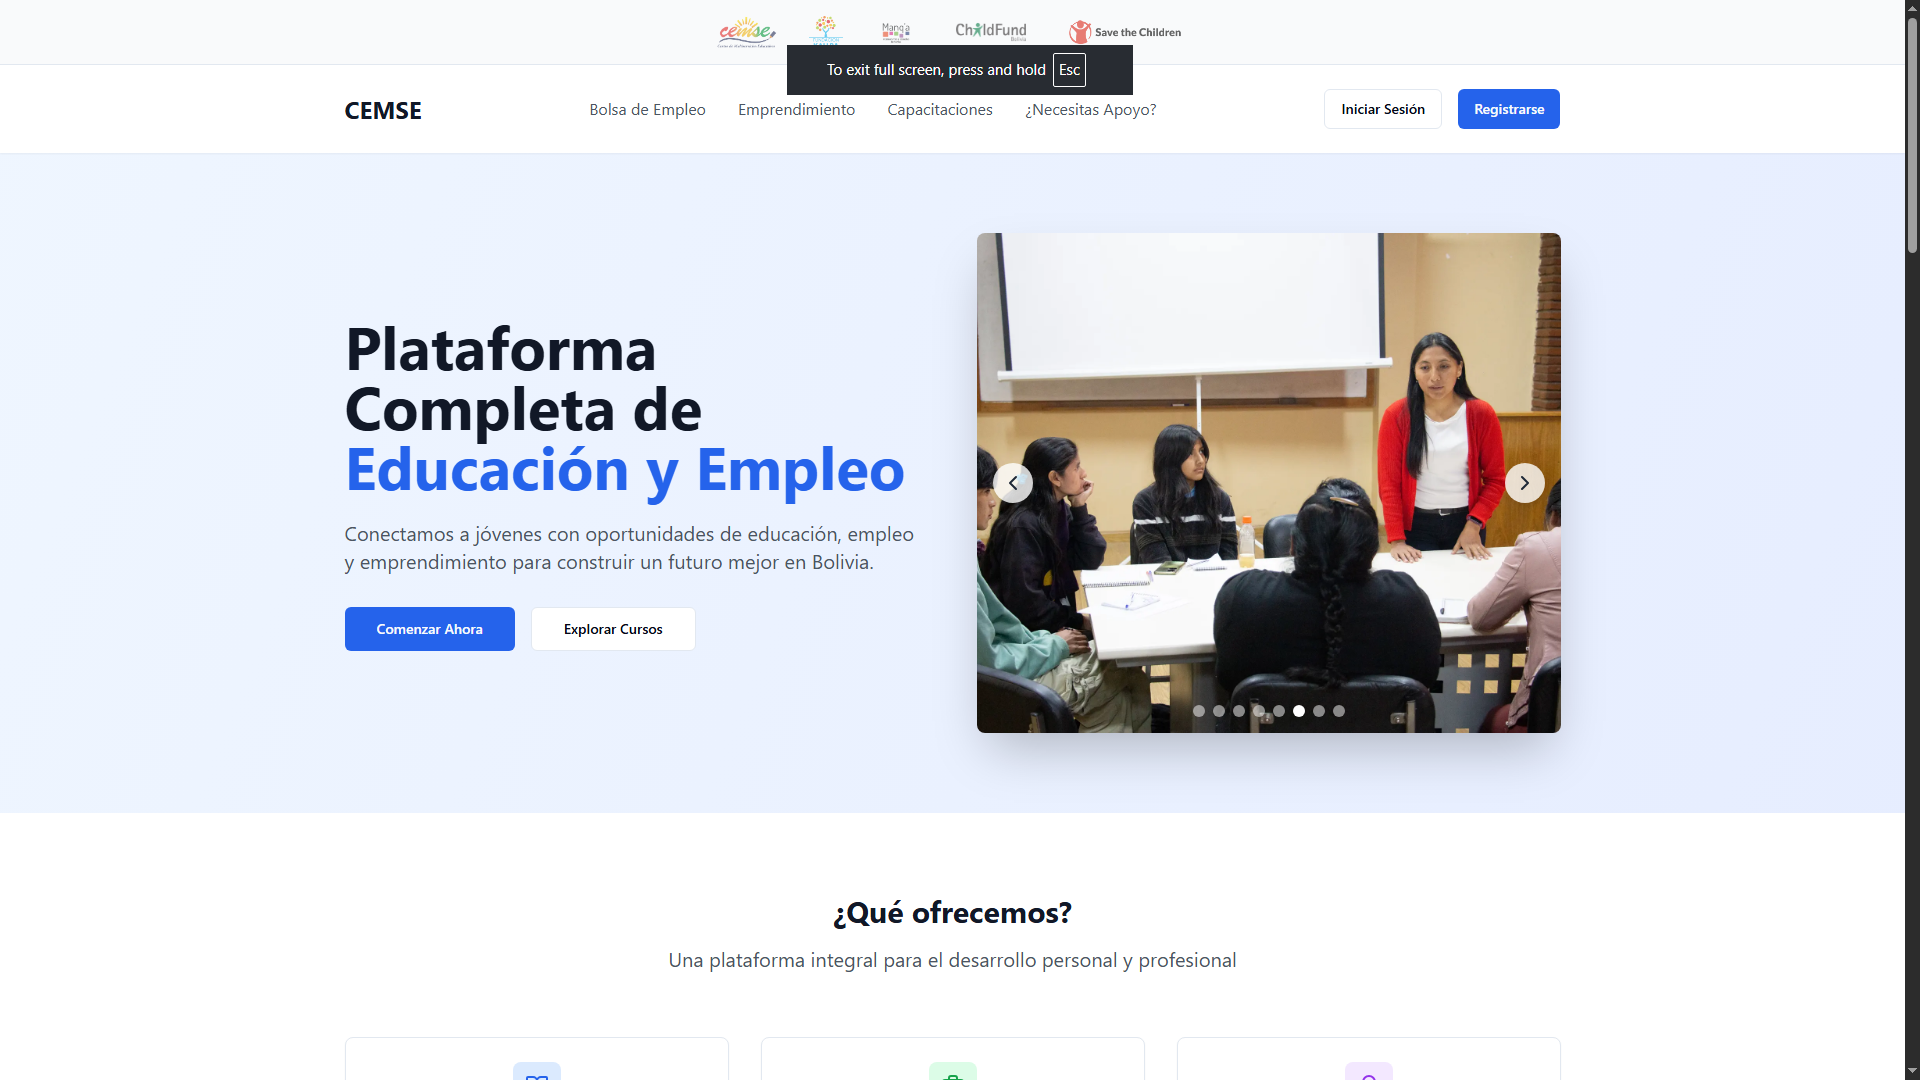
\includegraphics[width=0.9\textwidth]{screenshots/auth/landing-page.png}
    \caption{Página de inicio de la plataforma CEMSE}
    \label{fig:landing-page}
\end{figure}

\subsubsection{Inicio de Sesión}
\begin{figure}[H]
    \centering
    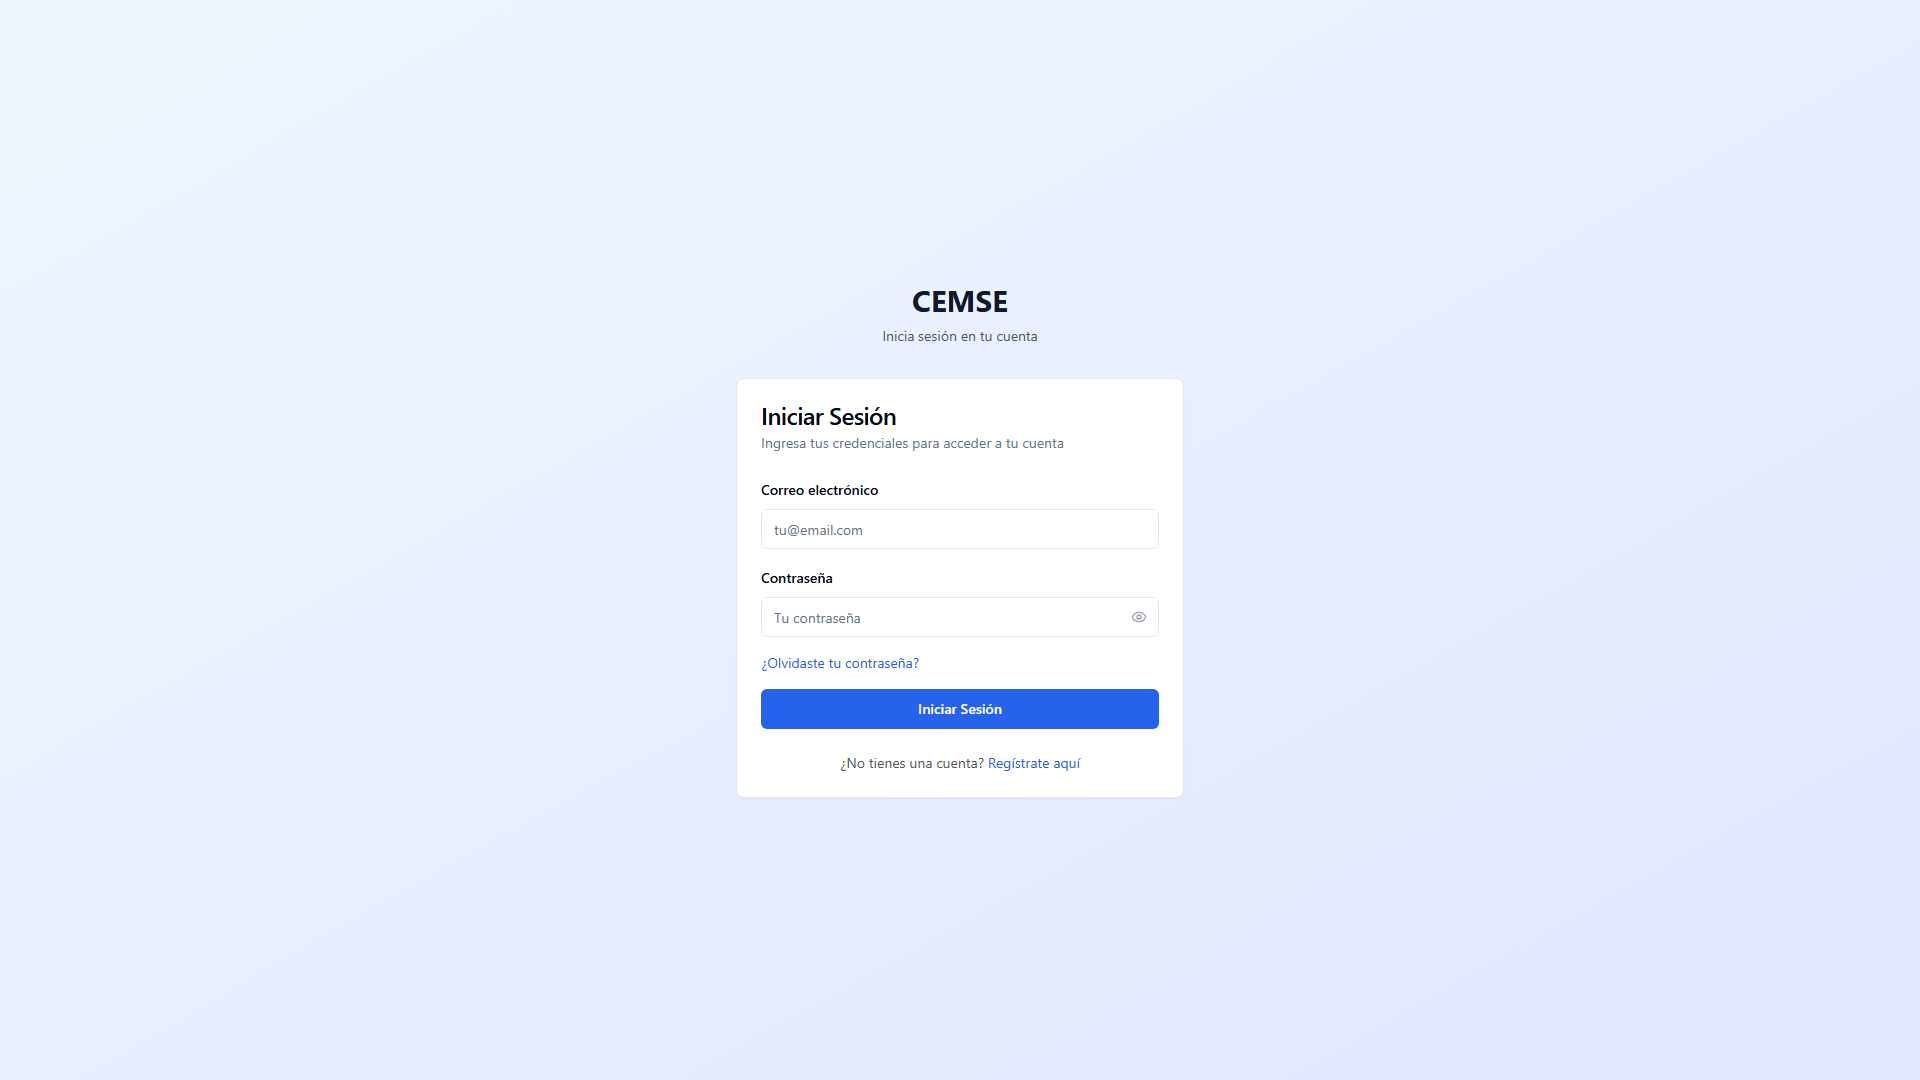
\includegraphics[width=0.6\textwidth]{screenshots/auth/sign-in.png}
    \caption{Formulario de inicio de sesión}
    \label{fig:sign-in}
\end{figure}

\subsubsection{Registro de Usuario}
\begin{figure}[H]
    \centering
    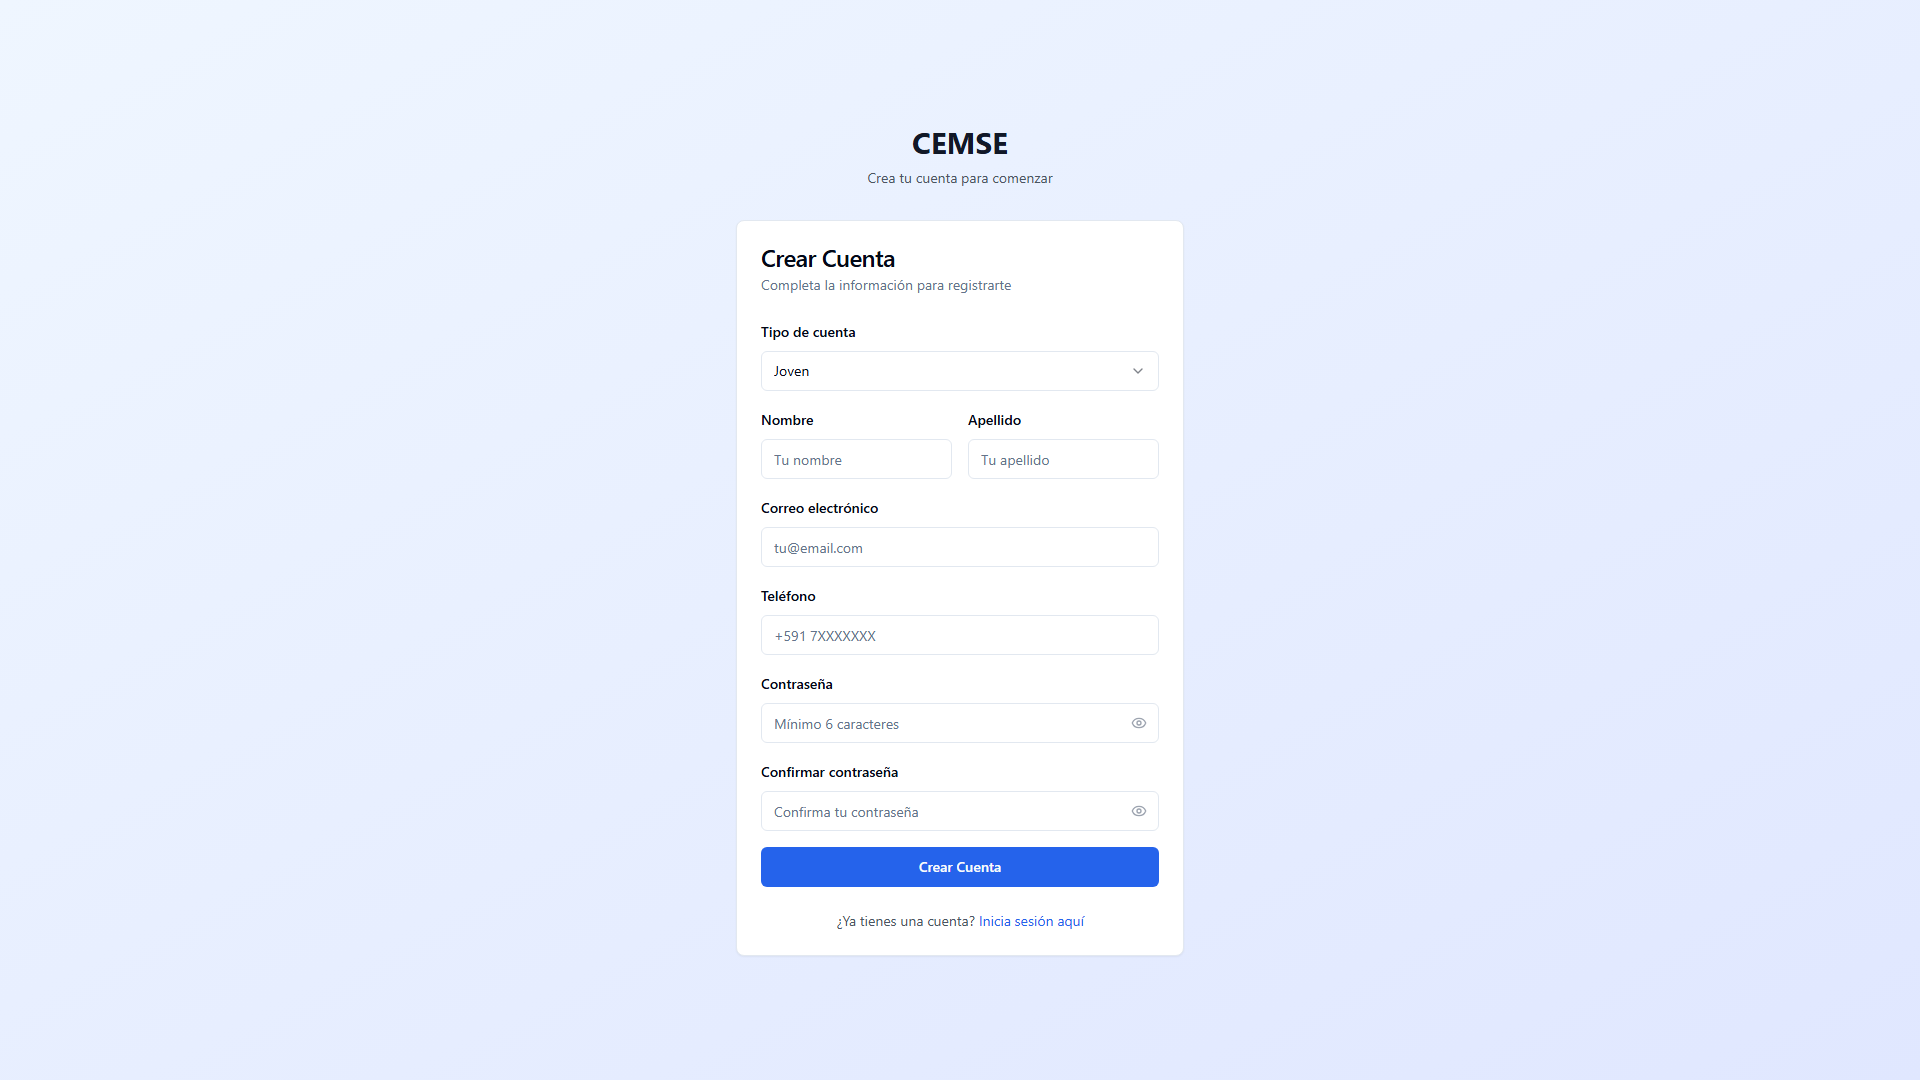
\includegraphics[width=0.6\textwidth]{screenshots/auth/sign-up.png}
    \caption{Formulario de registro de nuevos usuarios}
    \label{fig:sign-up}
\end{figure}

\subsection{Flujo de Usuario Joven (YOUTH)}

\subsubsection{Dashboard Principal}
\begin{figure}[H]
    \centering
    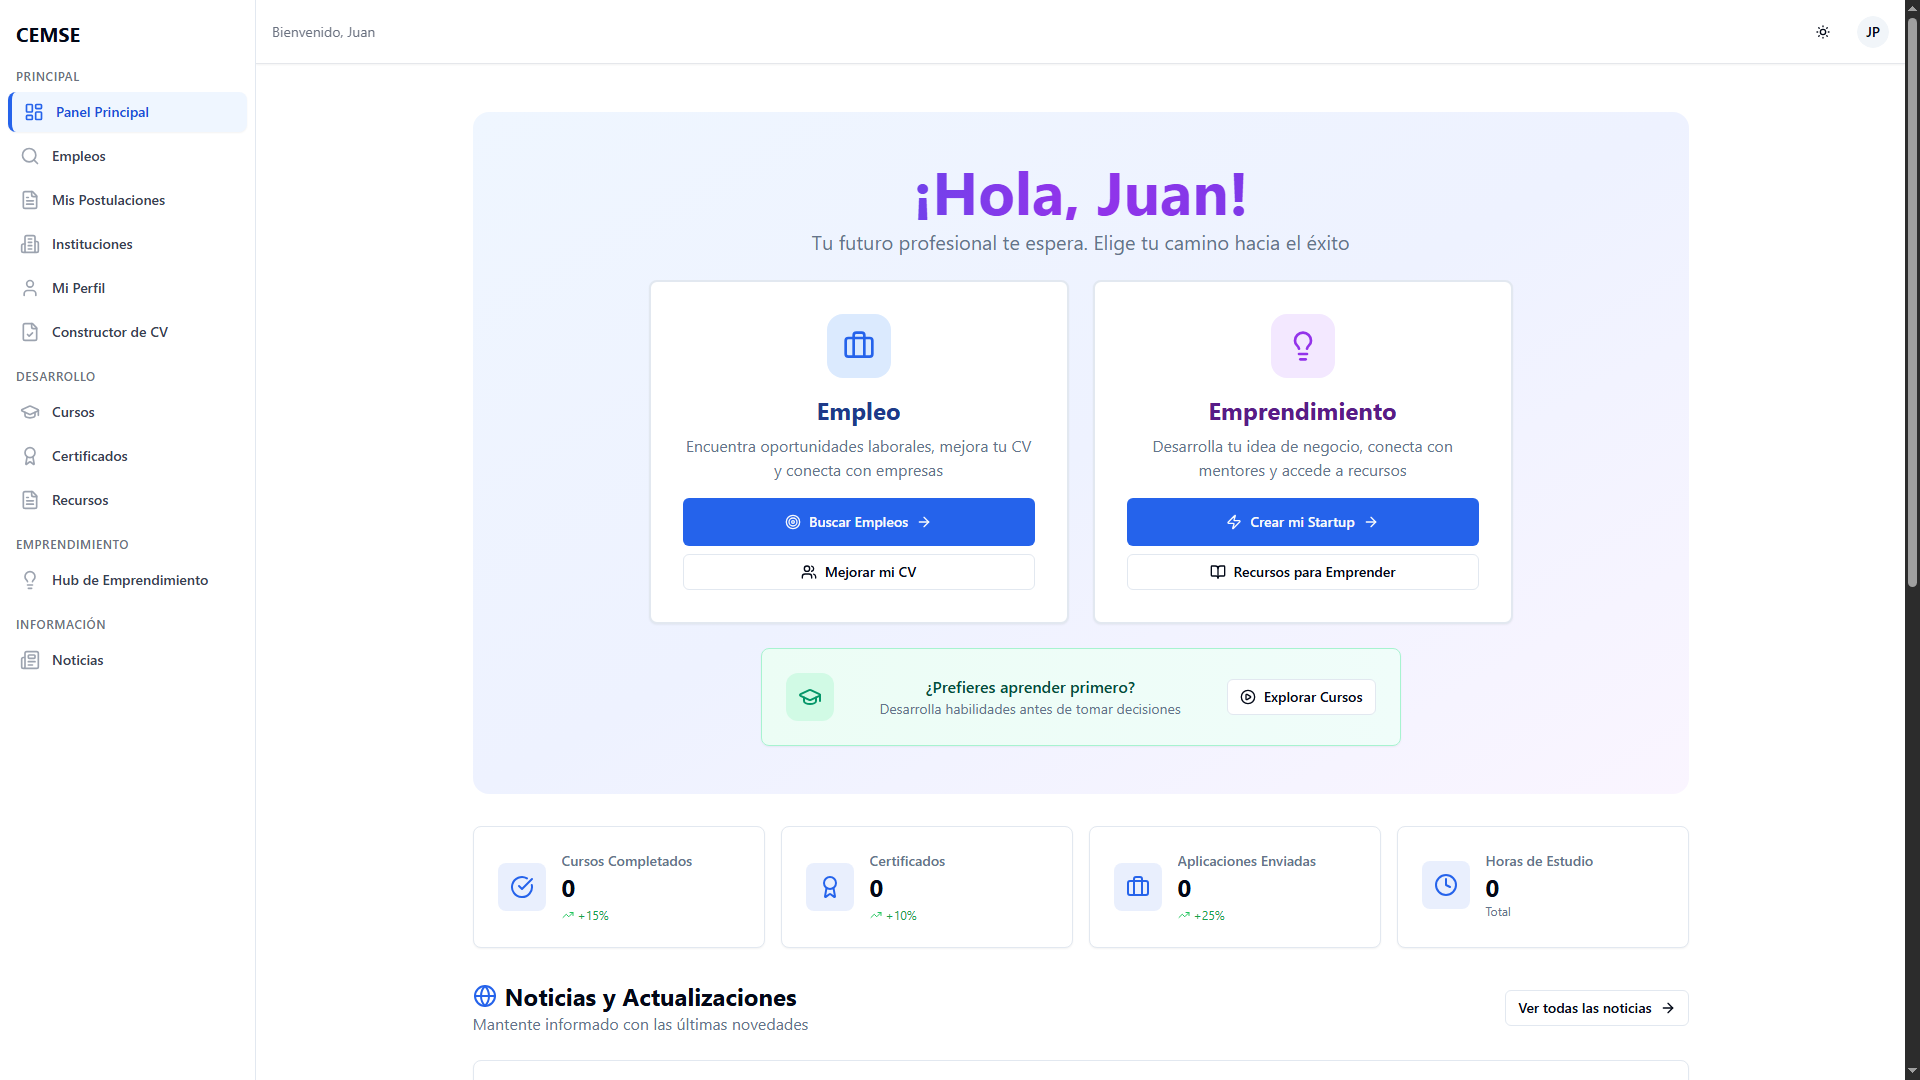
\includegraphics[width=0.9\textwidth]{screenshots/youth/dashboard.png}
    \caption{Dashboard principal para usuarios jóvenes}
    \label{fig:youth-dashboard}
\end{figure}

\subsubsection{Búsqueda de Empleos}
\begin{figure}[H]
    \centering
    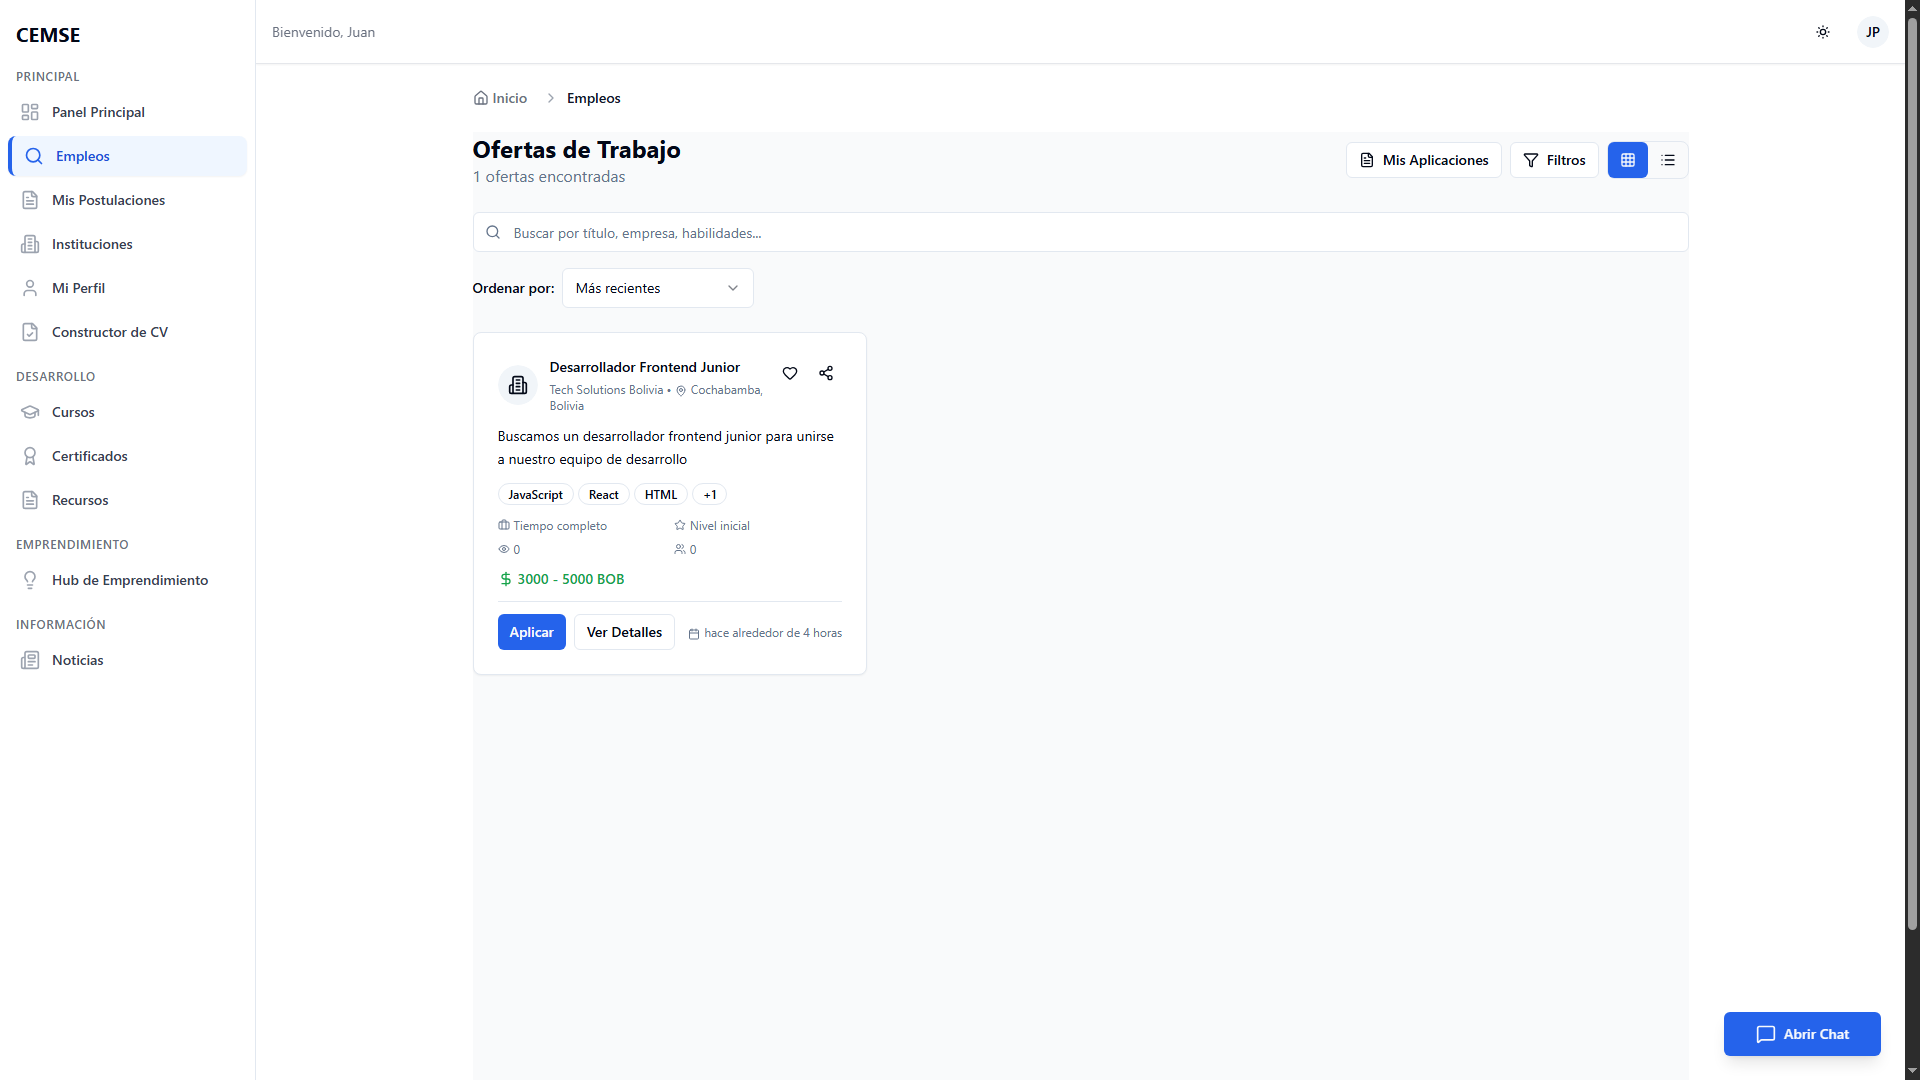
\includegraphics[width=0.9\textwidth]{screenshots/youth/jobs-search.png}
    \caption{Portal de búsqueda de empleos}
    \label{fig:youth-jobs}
\end{figure}

\subsubsection{Detalle de Oferta Laboral}
\begin{figure}[H]
    \centering
    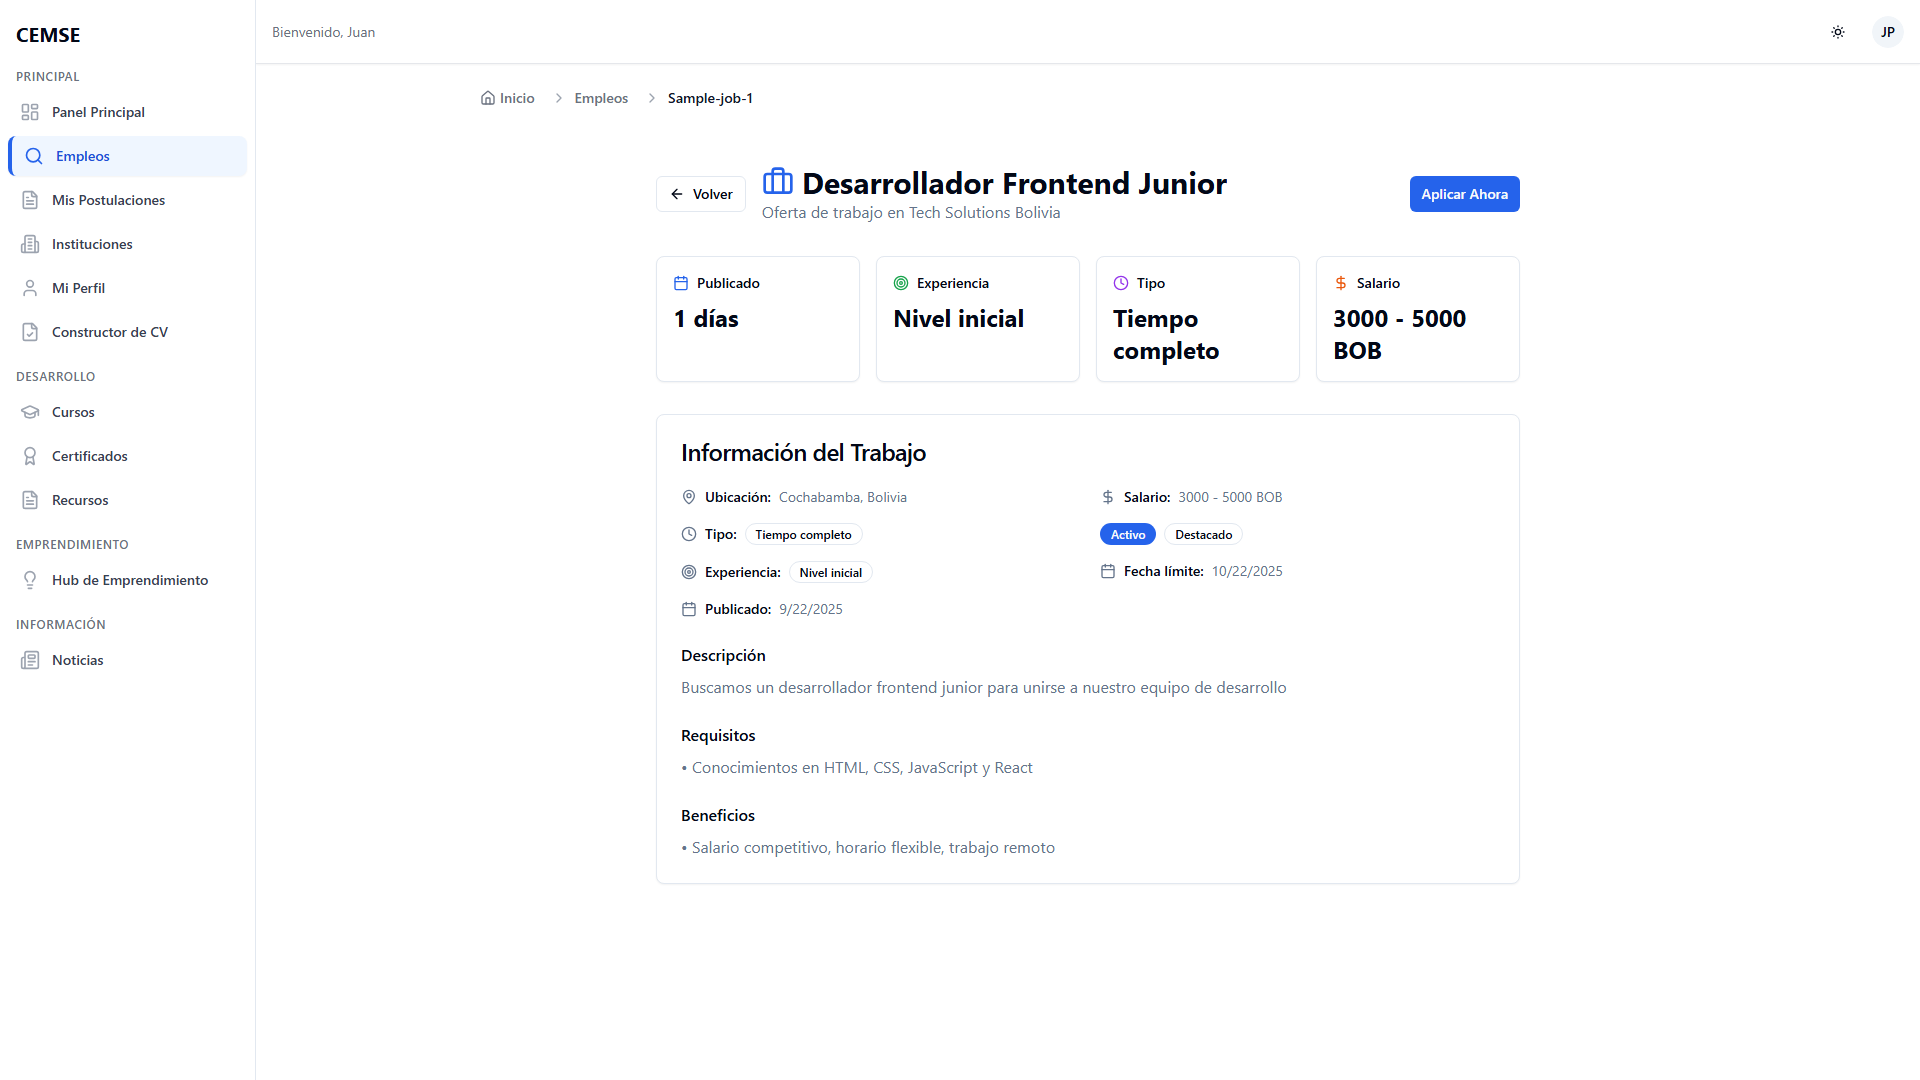
\includegraphics[width=0.9\textwidth]{screenshots/youth/job-detail.png}
    \caption{Detalle de una oferta laboral específica}
    \label{fig:youth-job-detail}
\end{figure}

\subsubsection{Aplicación a Empleo}
\begin{figure}[H]
    \centering
    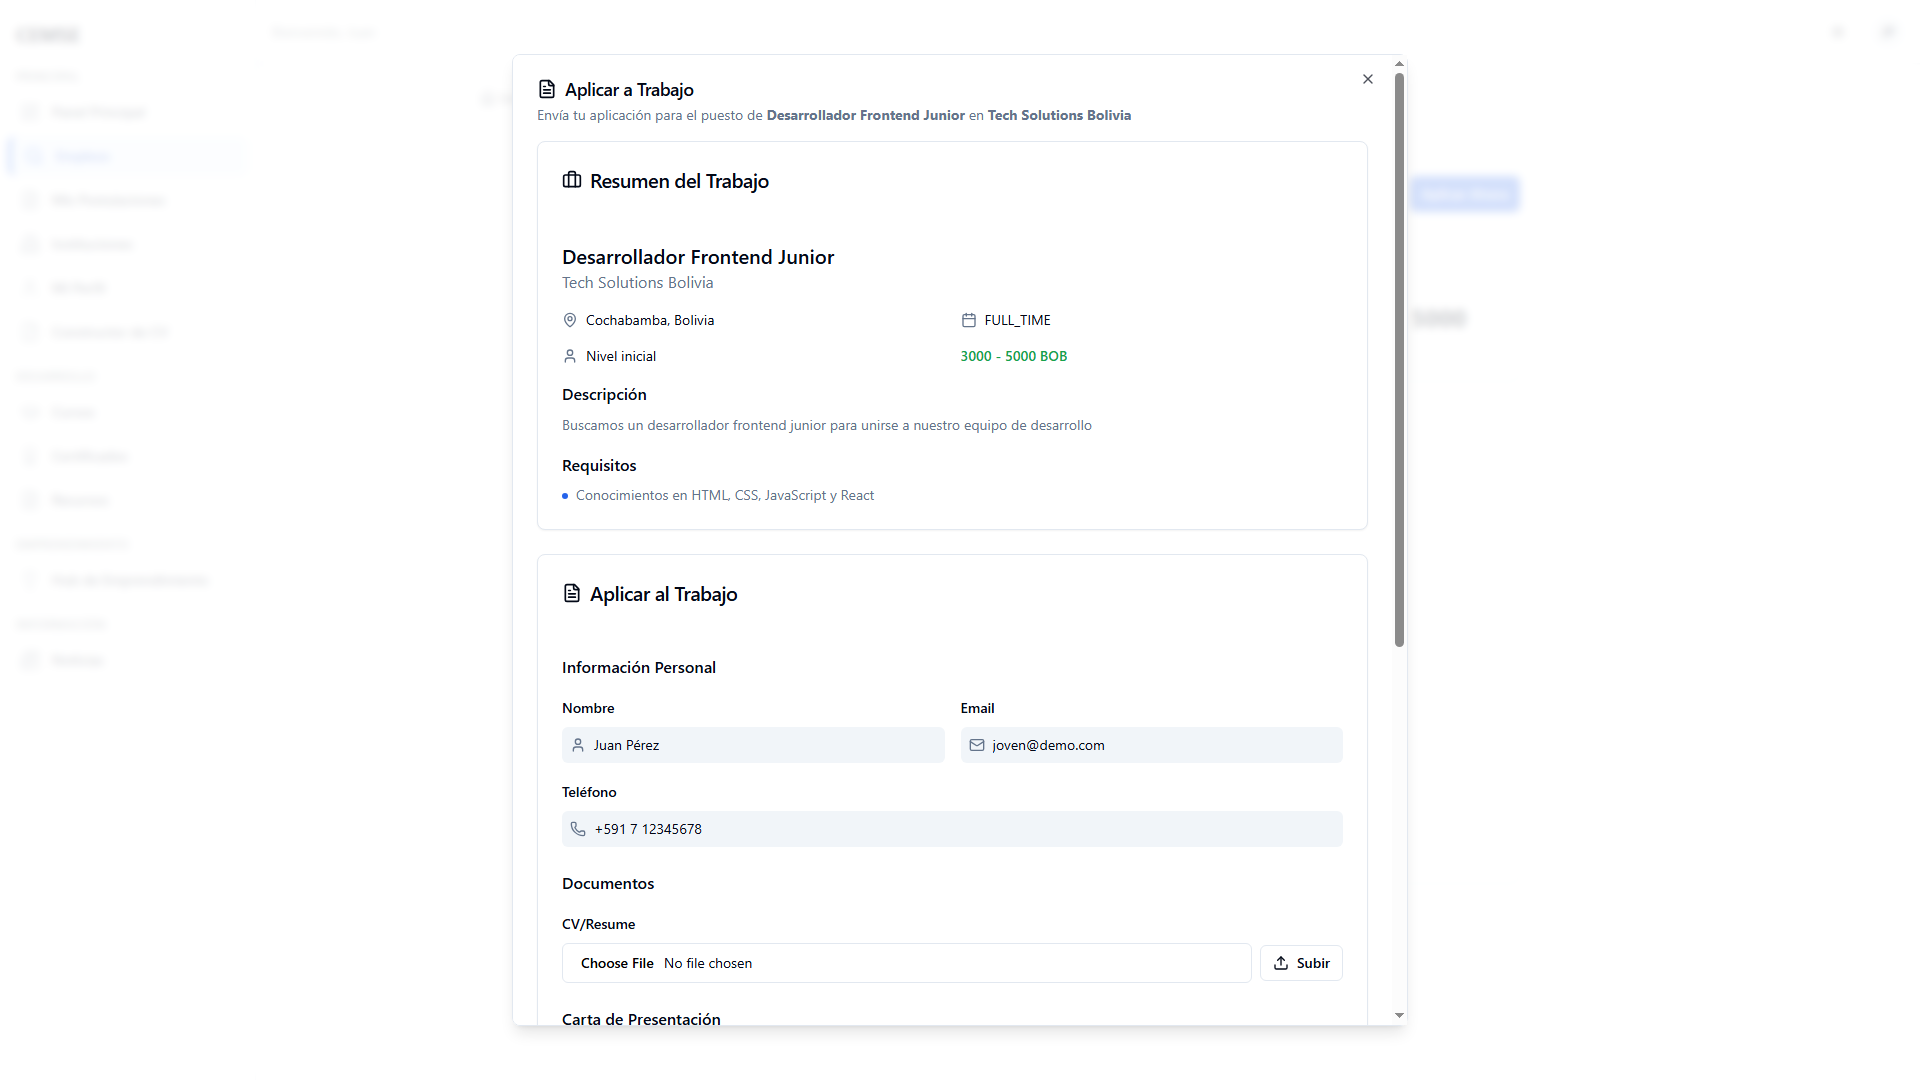
\includegraphics[width=0.9\textwidth]{screenshots/youth/job-apply.png}
    \caption{Formulario de aplicación a empleo}
    \label{fig:youth-job-apply}
\end{figure}

\subsubsection{Mis Postulaciones}
\begin{figure}[H]
    \centering
    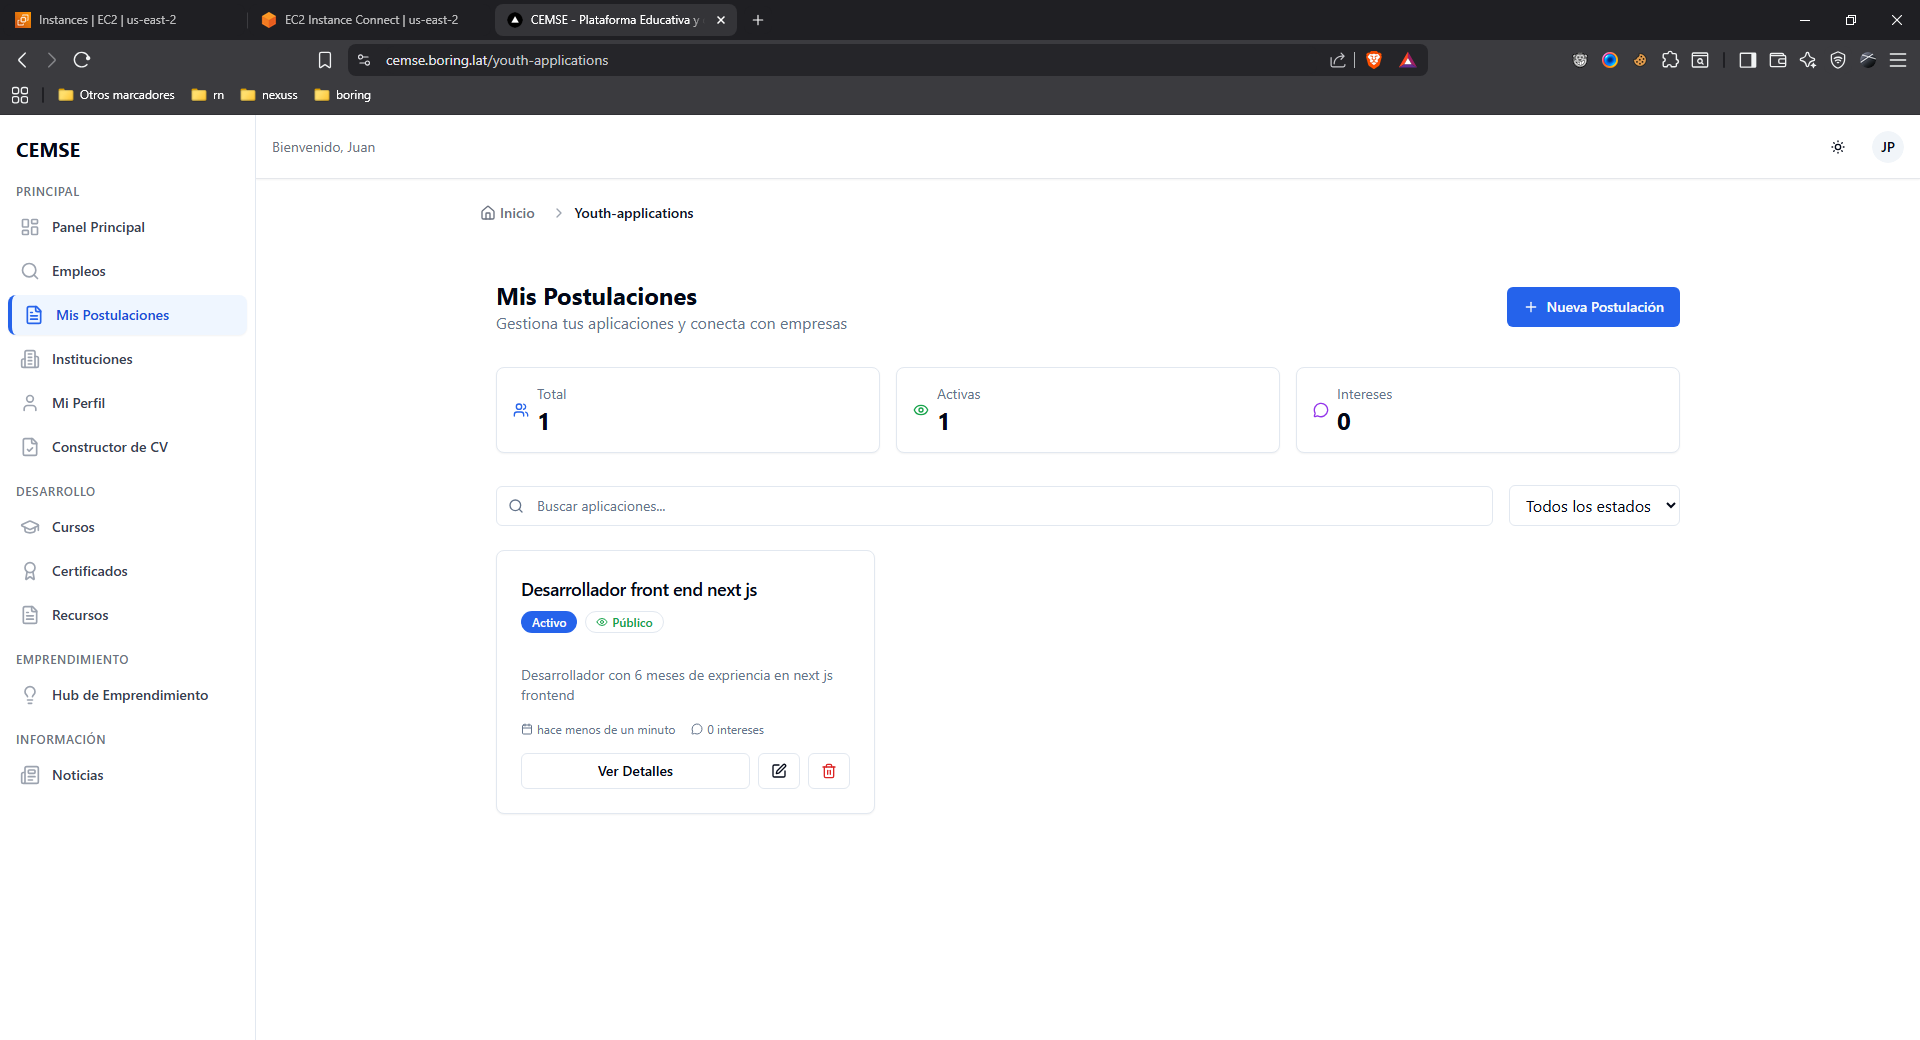
\includegraphics[width=0.9\textwidth]{screenshots/youth/my-applications.png}
    \caption{Panel de seguimiento de postulaciones}
    \label{fig:youth-applications}
\end{figure}

\subsubsection{Catálogo de Cursos}
\begin{figure}[H]
    \centering
    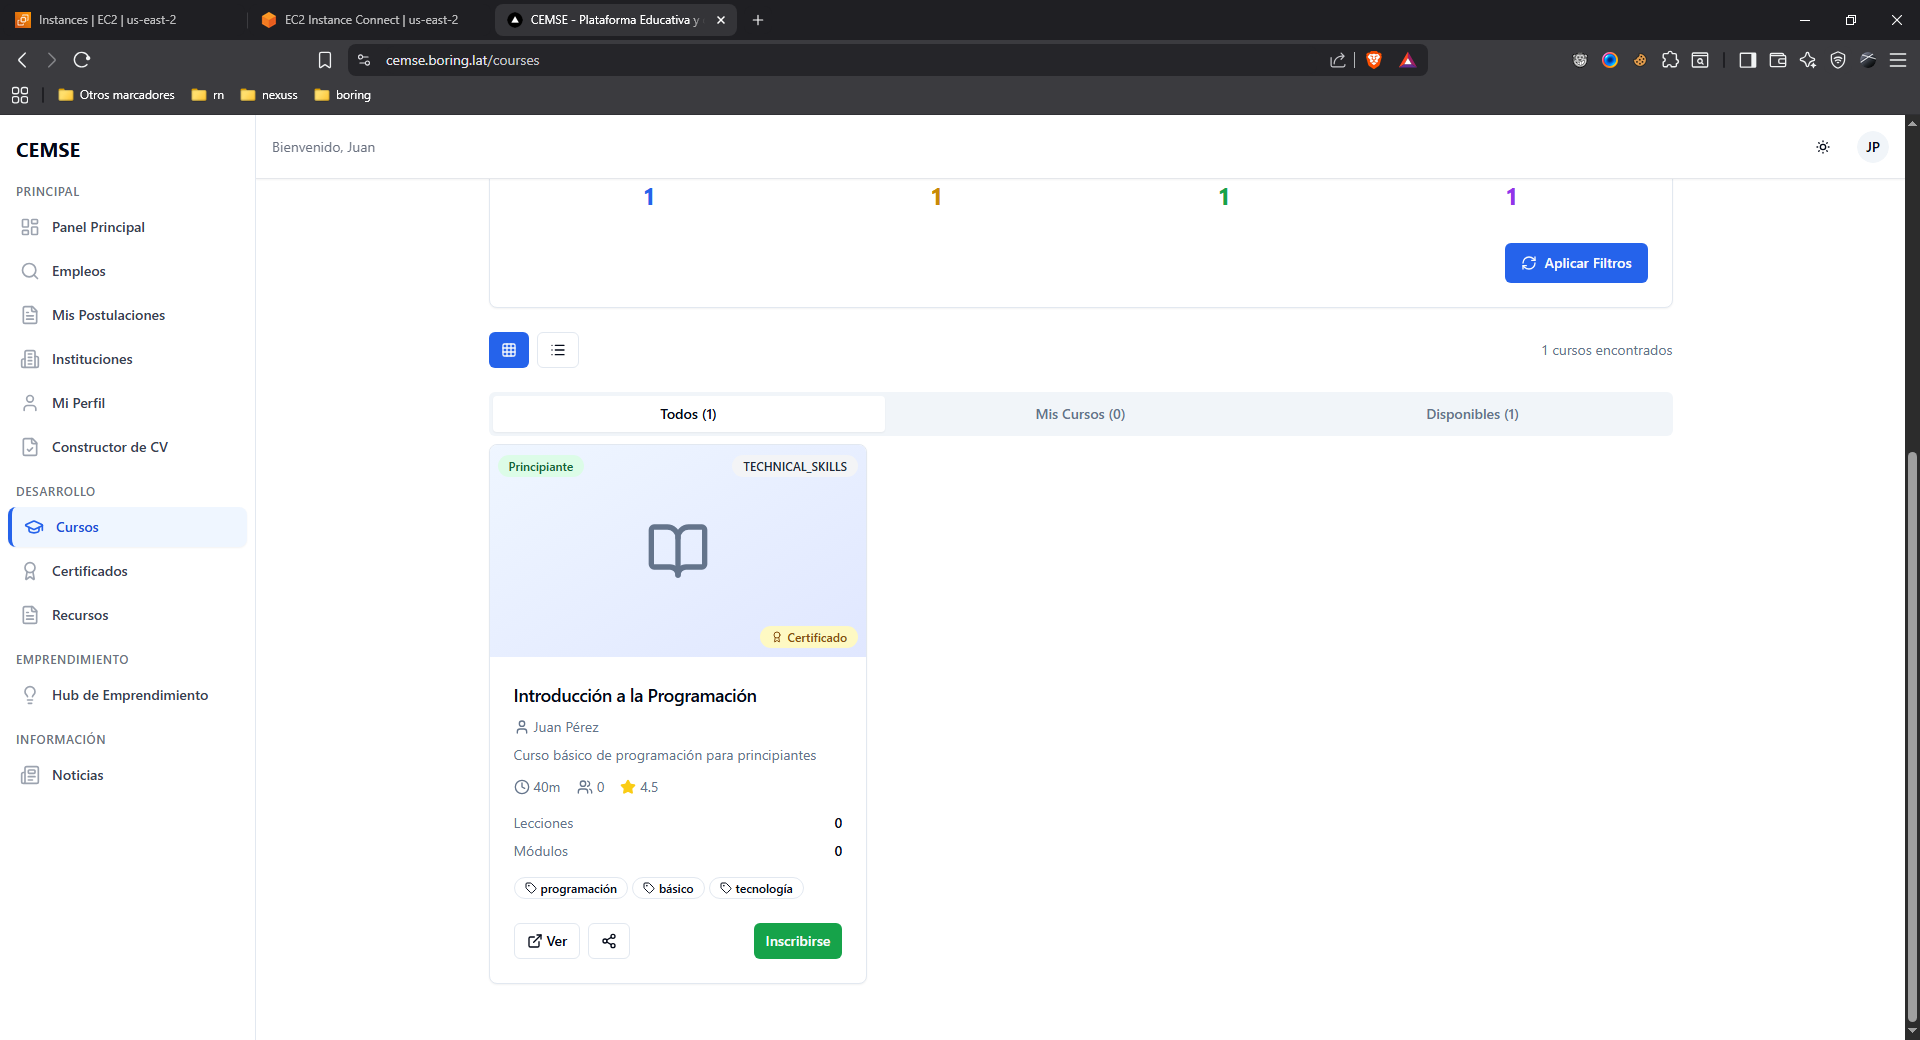
\includegraphics[width=0.9\textwidth]{screenshots/youth/courses.png}
    \caption{Catálogo de cursos disponibles}
    \label{fig:youth-courses}
\end{figure}

\subsubsection{Constructor de CV}
\begin{figure}[H]
    \centering
    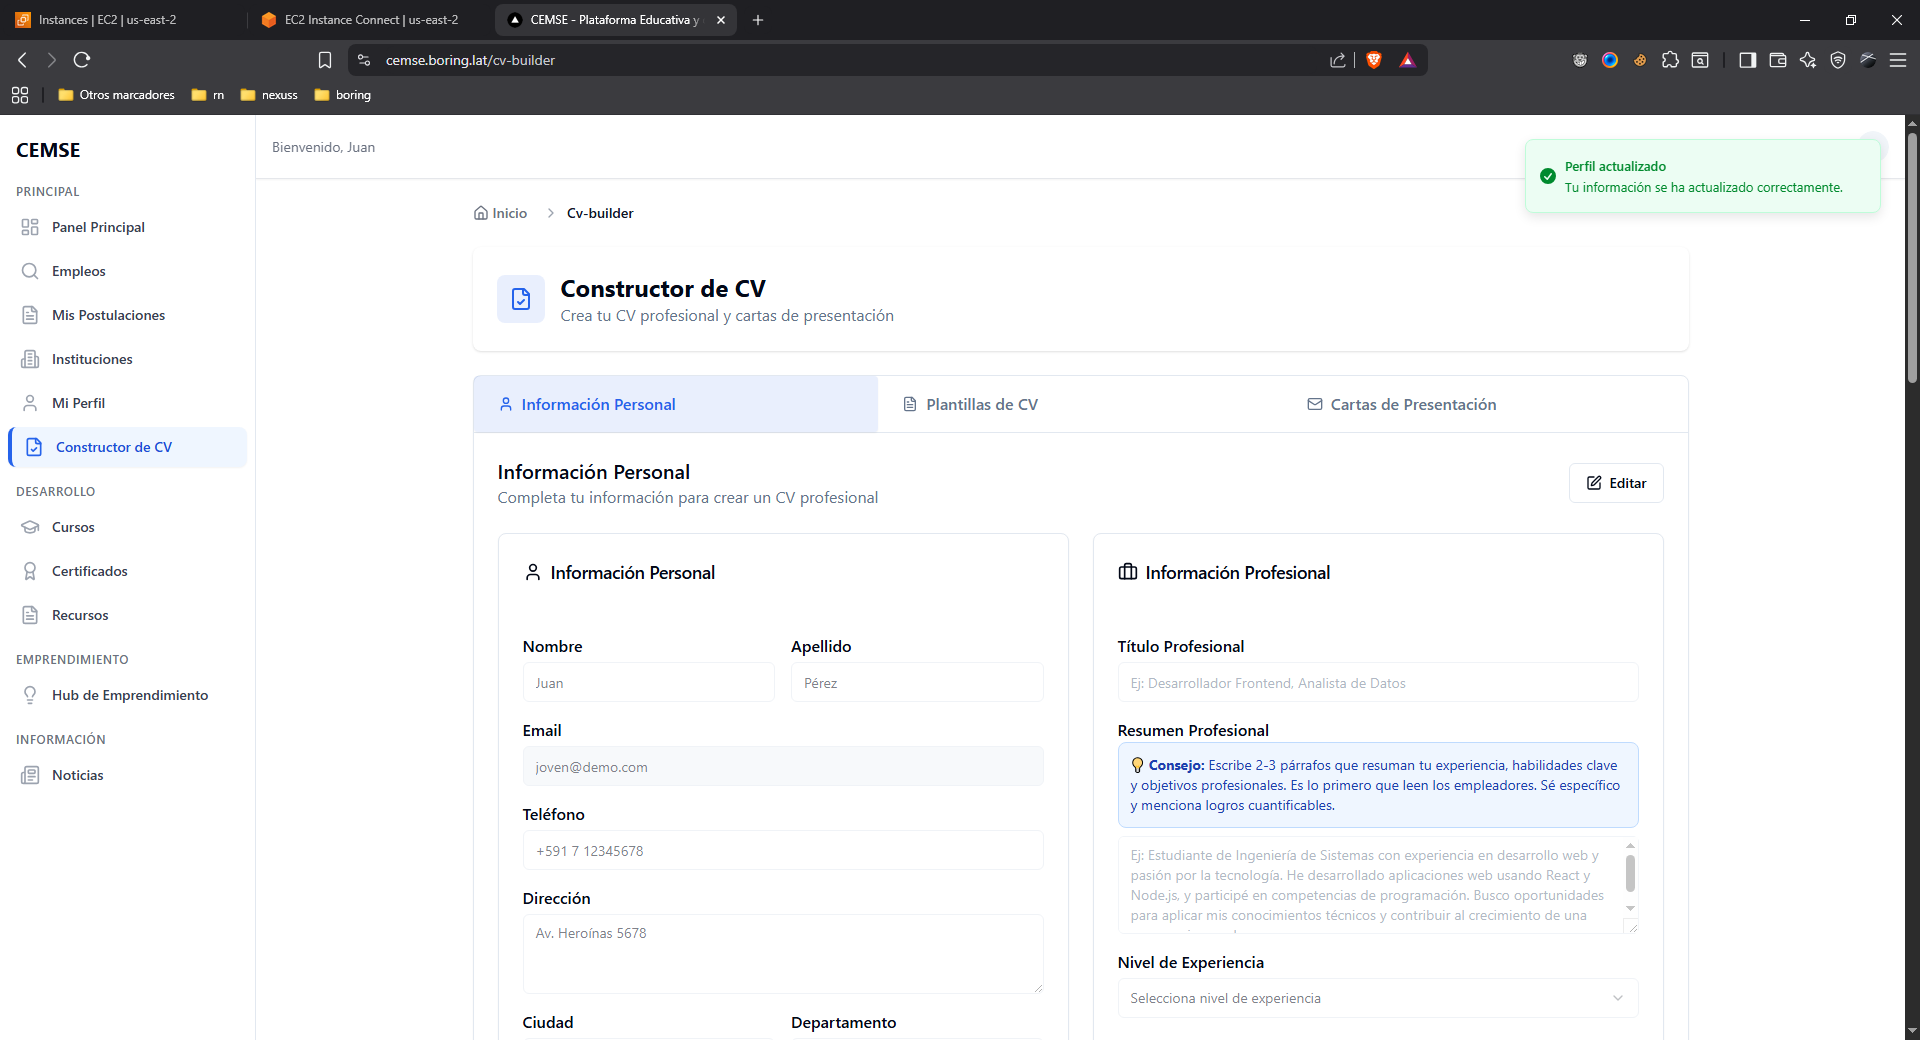
\includegraphics[width=0.9\textwidth]{screenshots/youth/cv-builder.png}
    \caption{Herramienta de construcción de currículum}
    \label{fig:youth-cv-builder}
\end{figure}

\subsubsection{Perfil de Usuario}
\begin{figure}[H]
    \centering
    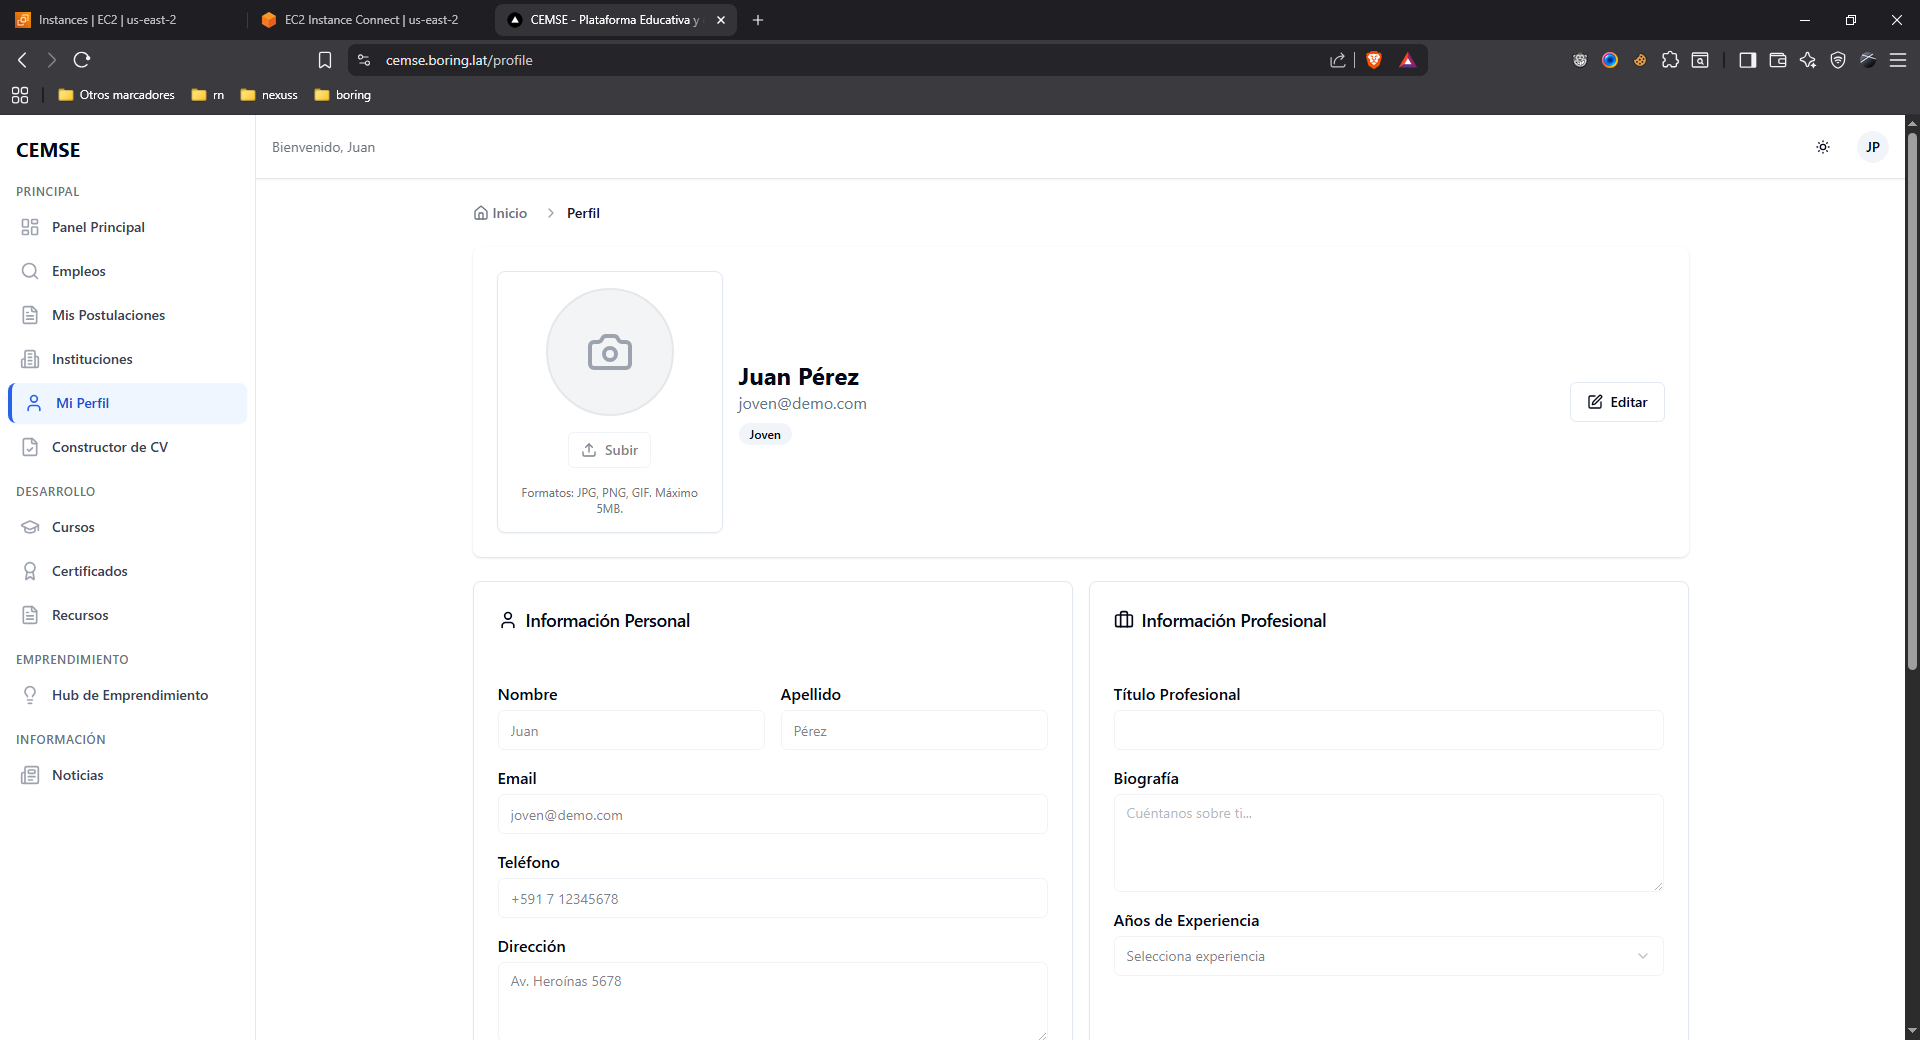
\includegraphics[width=0.9\textwidth]{screenshots/youth/profile.png}
    \caption{Perfil personal del usuario}
    \label{fig:youth-profile}
\end{figure}

\subsubsection{Hub de Emprendimiento}
\begin{figure}[H]
    \centering
    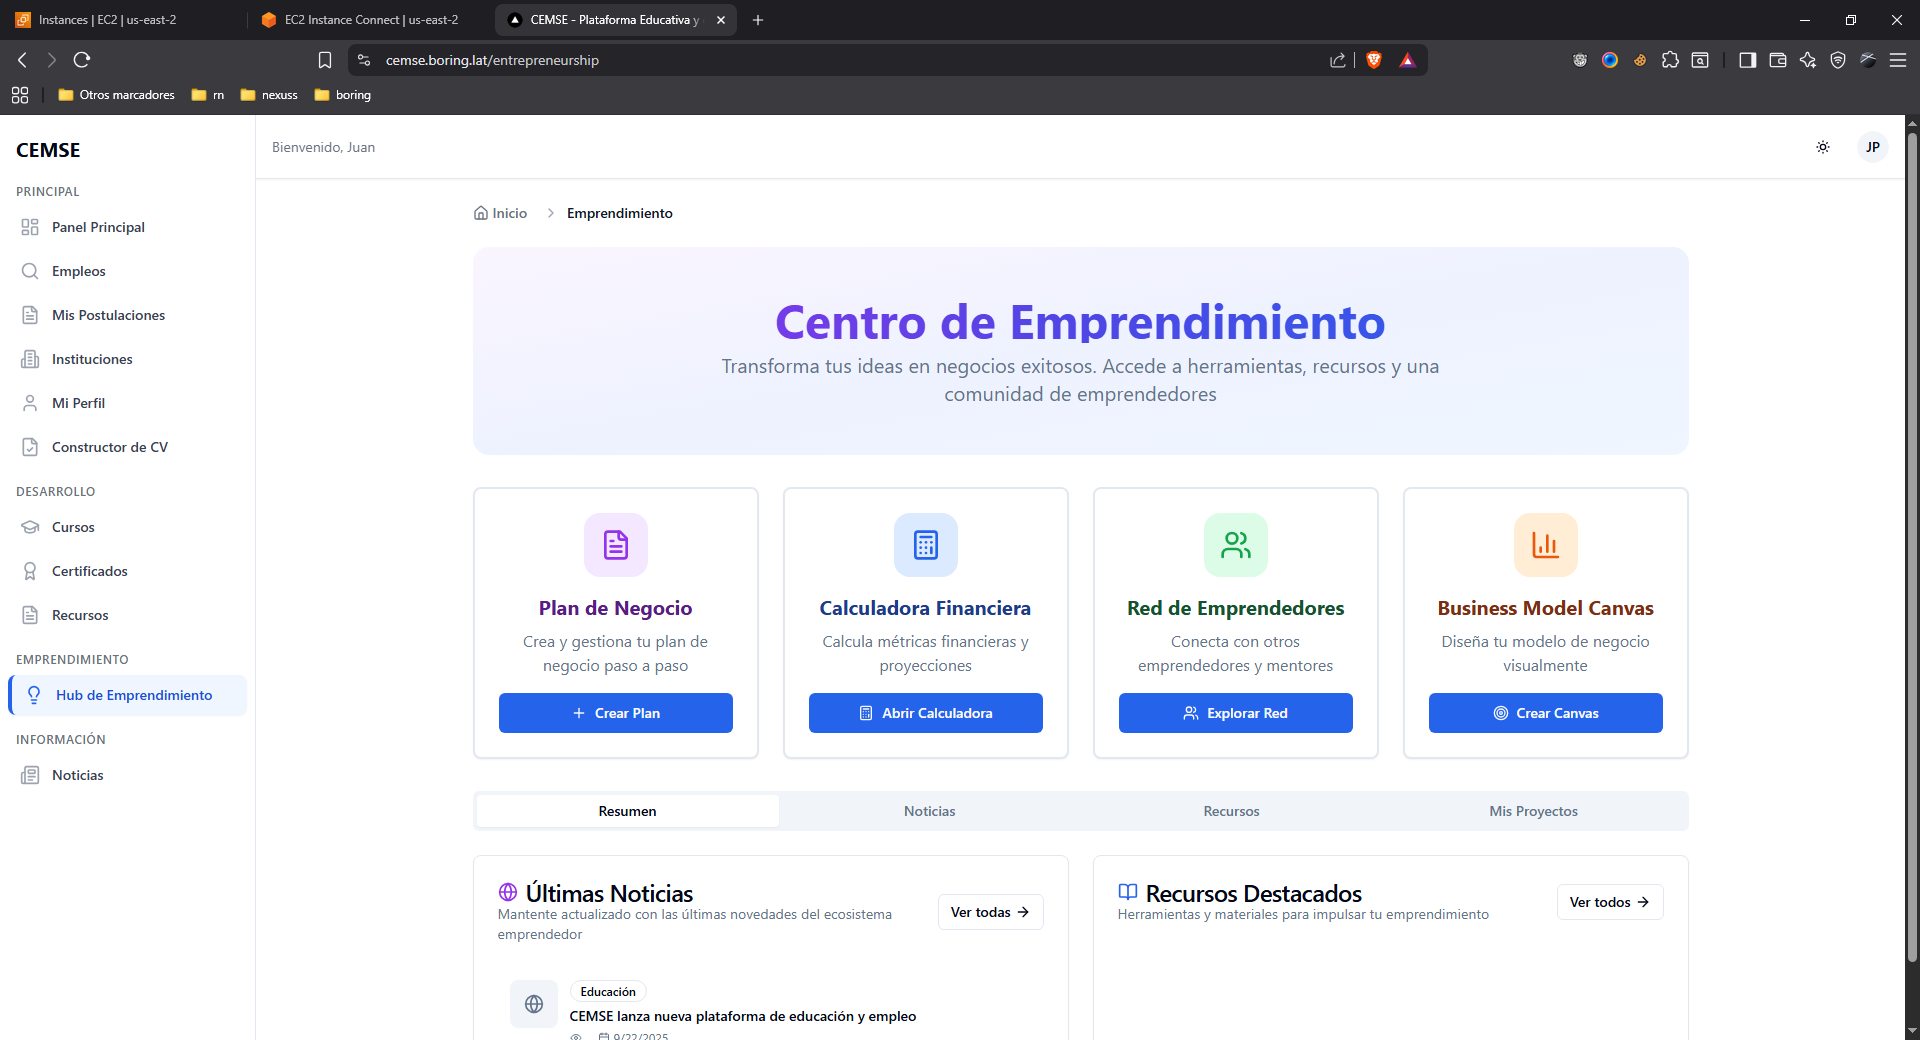
\includegraphics[width=0.9\textwidth]{screenshots/youth/entrepreneurship.png}
    \caption{Portal de emprendimiento y networking}
    \label{fig:youth-entrepreneurship}
\end{figure}

\subsection{Flujo de Usuario Empresa (COMPANIES)}

\subsubsection{Dashboard de Empresa}
\begin{figure}[H]
    \centering
    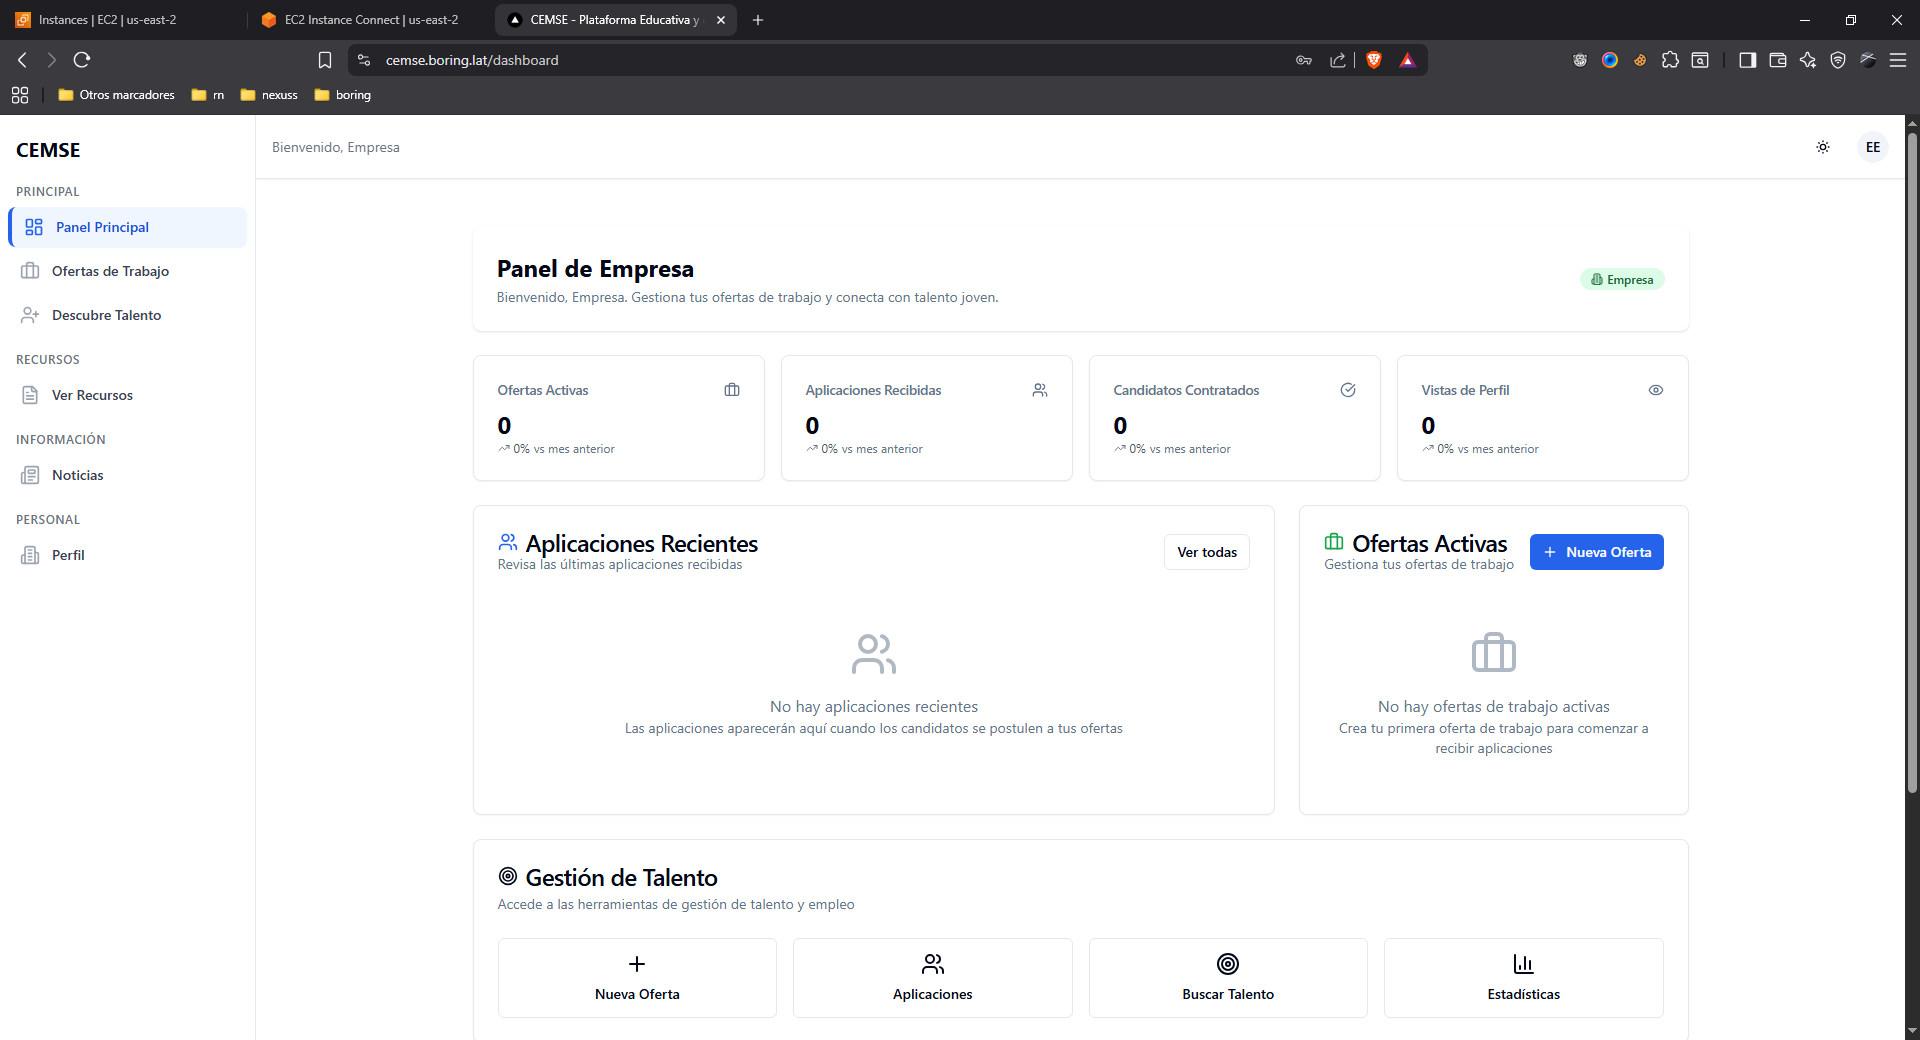
\includegraphics[width=0.9\textwidth]{screenshots/companies/dashboard.png}
    \caption{Dashboard principal para empresas}
    \label{fig:company-dashboard}
\end{figure}

\subsubsection{Creación de Oferta Laboral}
\begin{figure}[H]
    \centering
    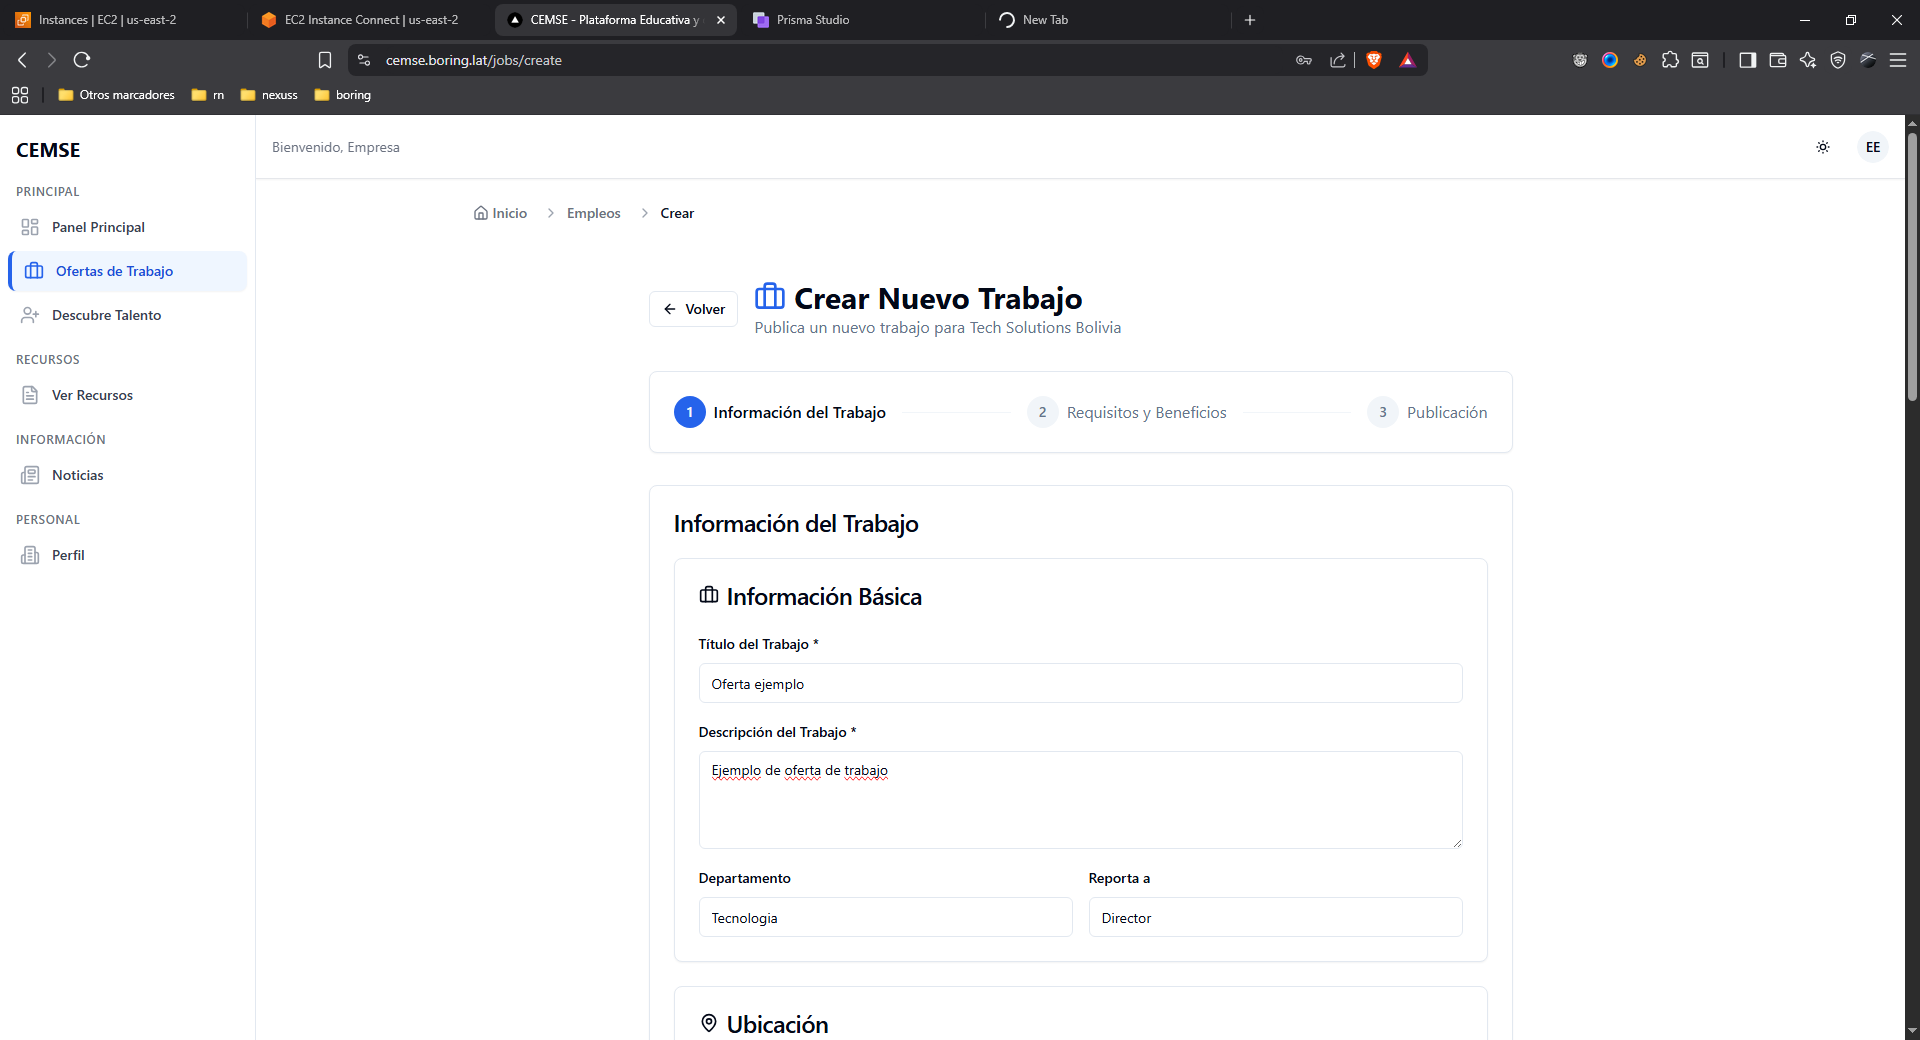
\includegraphics[width=0.9\textwidth]{screenshots/companies/create-job.png}
    \caption{Formulario de creación de oferta laboral}
    \label{fig:company-create-job}
\end{figure}

\subsubsection{Gestión de Empleos}
\begin{figure}[H]
    \centering
    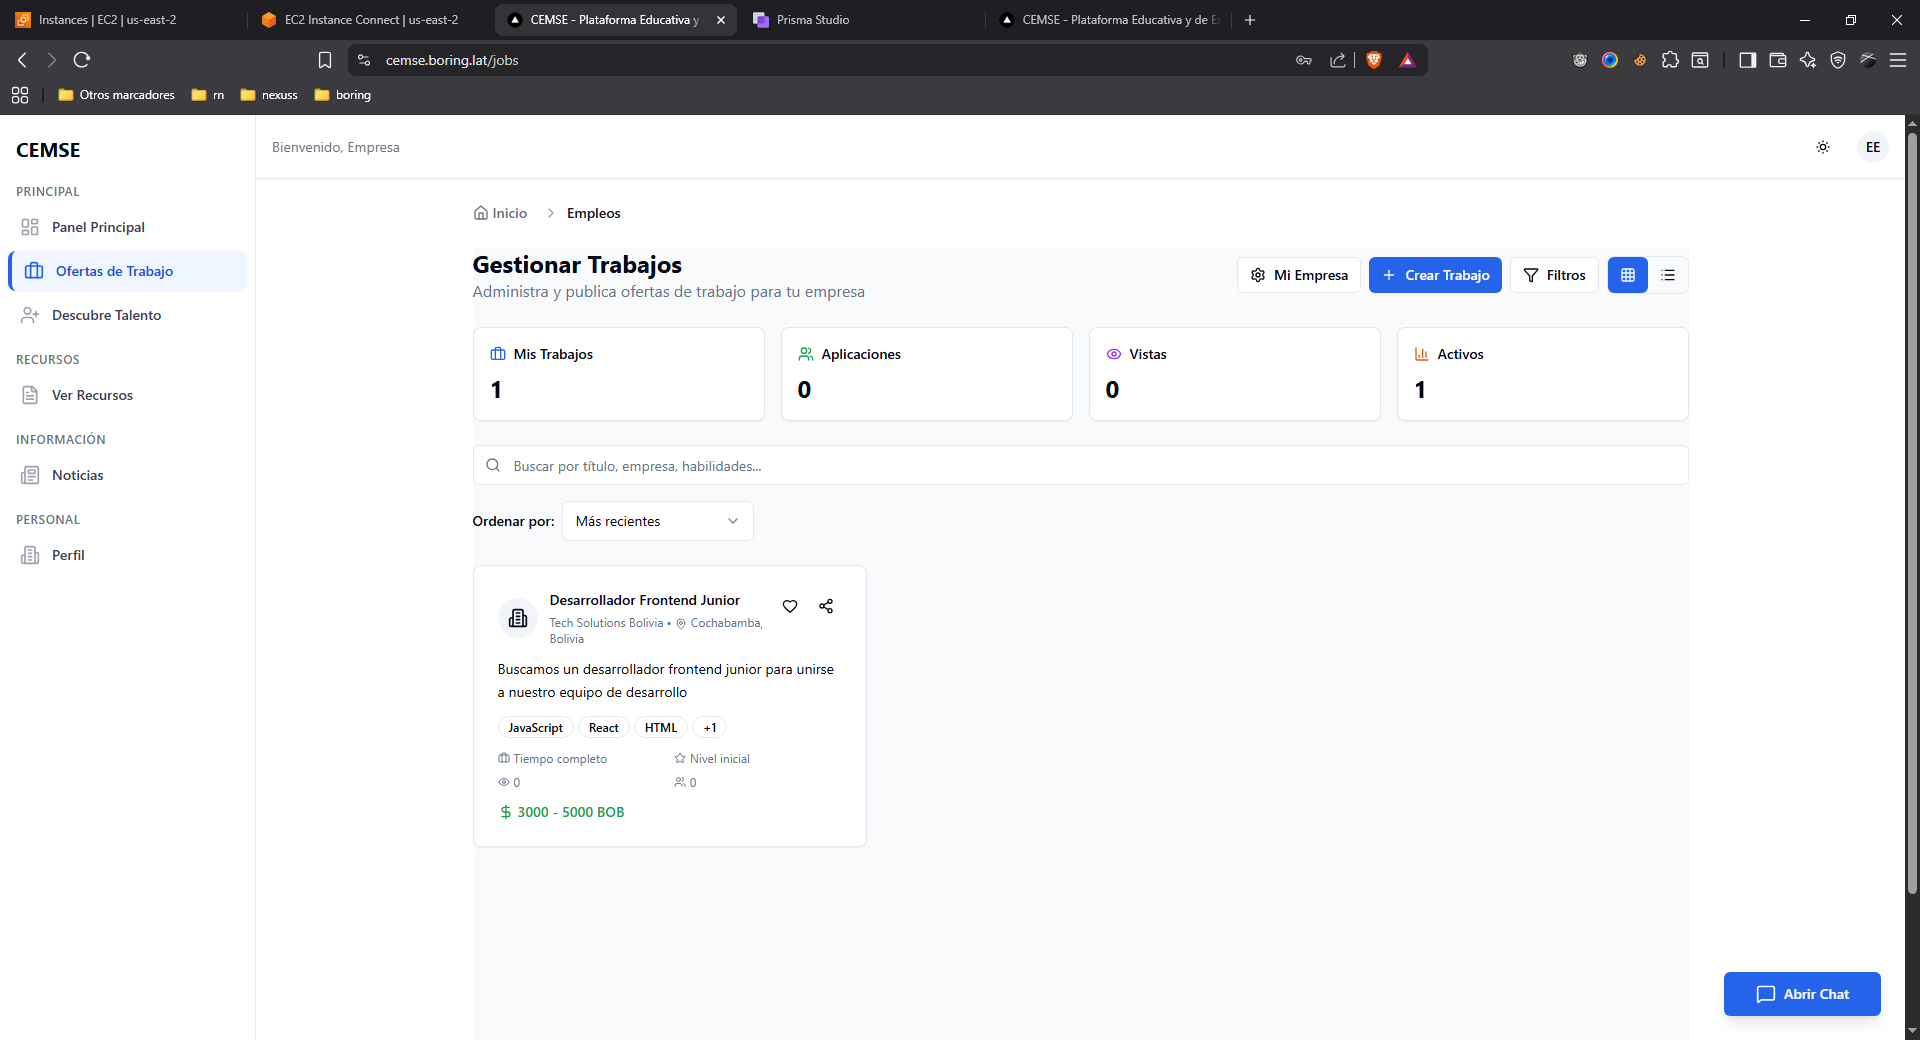
\includegraphics[width=0.9\textwidth]{screenshots/companies/job-management.png}
    \caption{Panel de gestión de ofertas laborales}
    \label{fig:company-jobs}
\end{figure}

\subsubsection{Descubrimiento de Talento}
\begin{figure}[H]
    \centering
    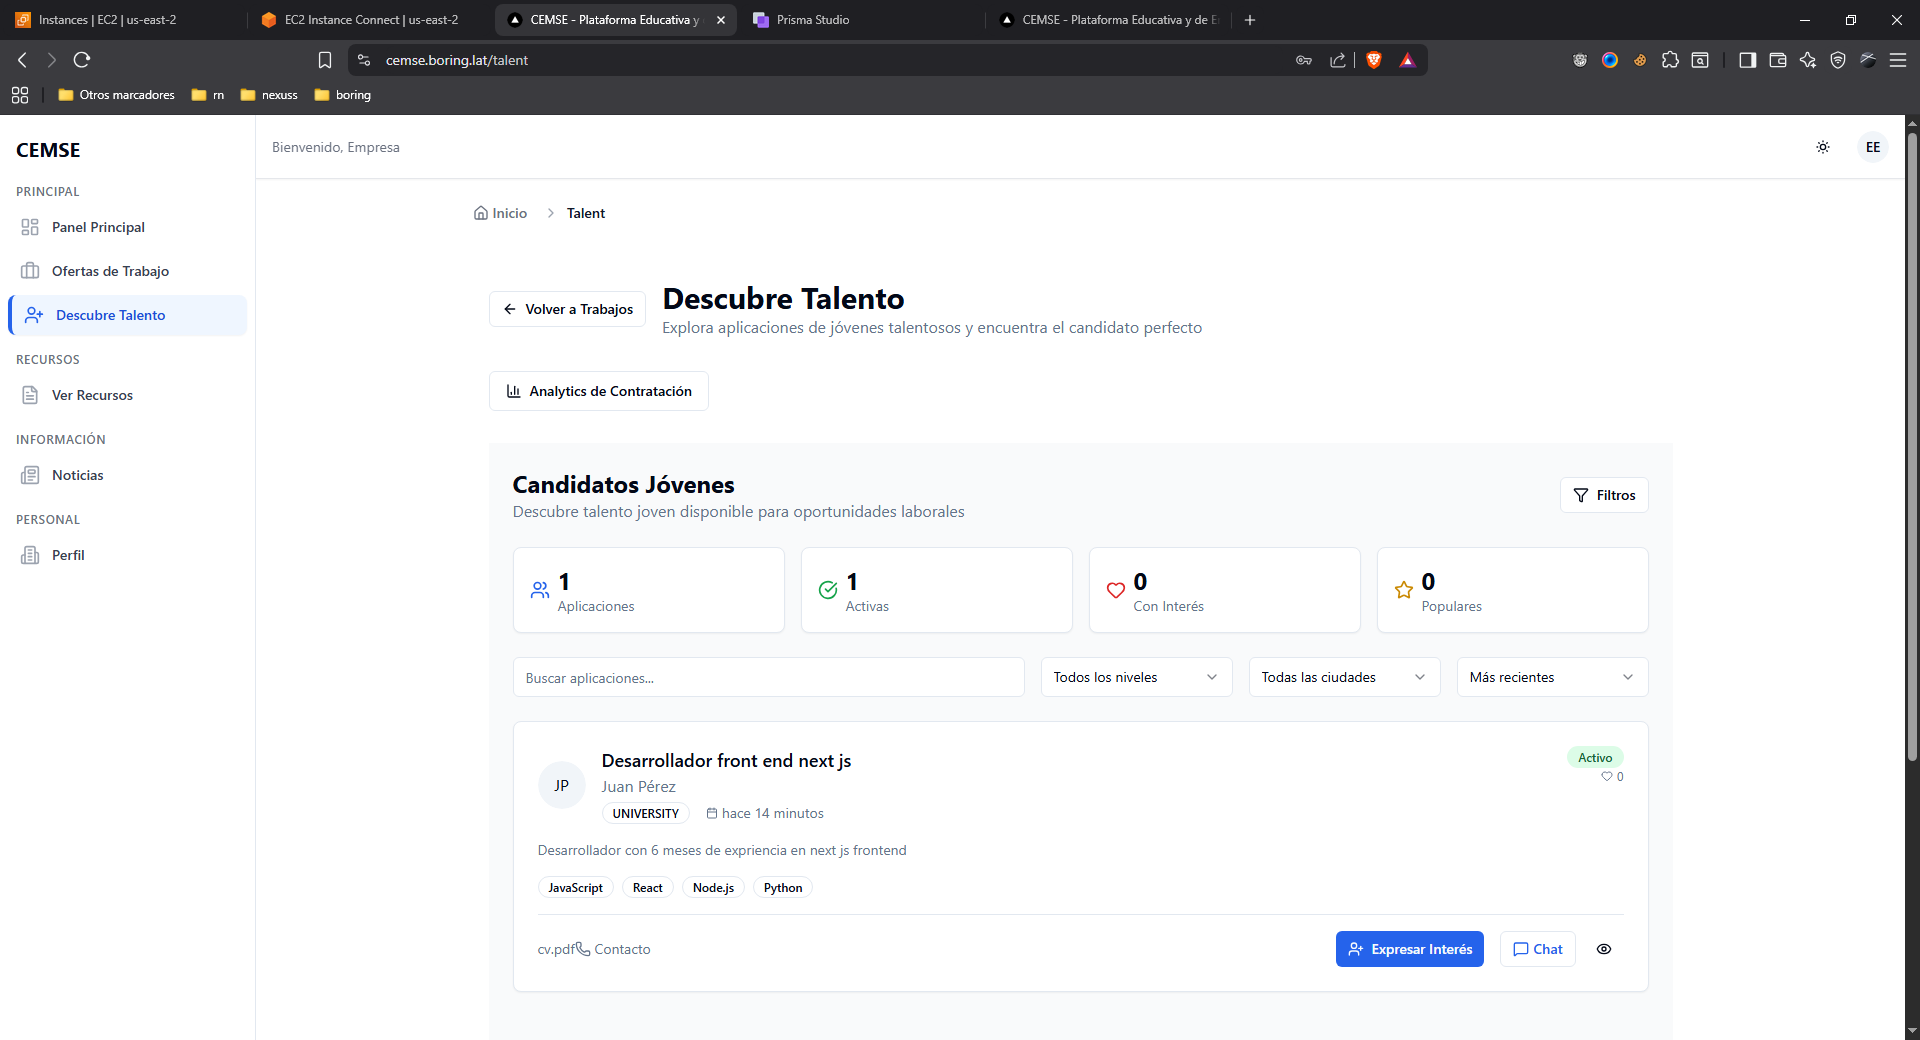
\includegraphics[width=0.9\textwidth]{screenshots/companies/talent-discovery.png}
    \caption{Portal de descubrimiento de talento}
    \label{fig:company-talent}
\end{figure}

\subsubsection{Perfil de Empresa}
\begin{figure}[H]
    \centering
    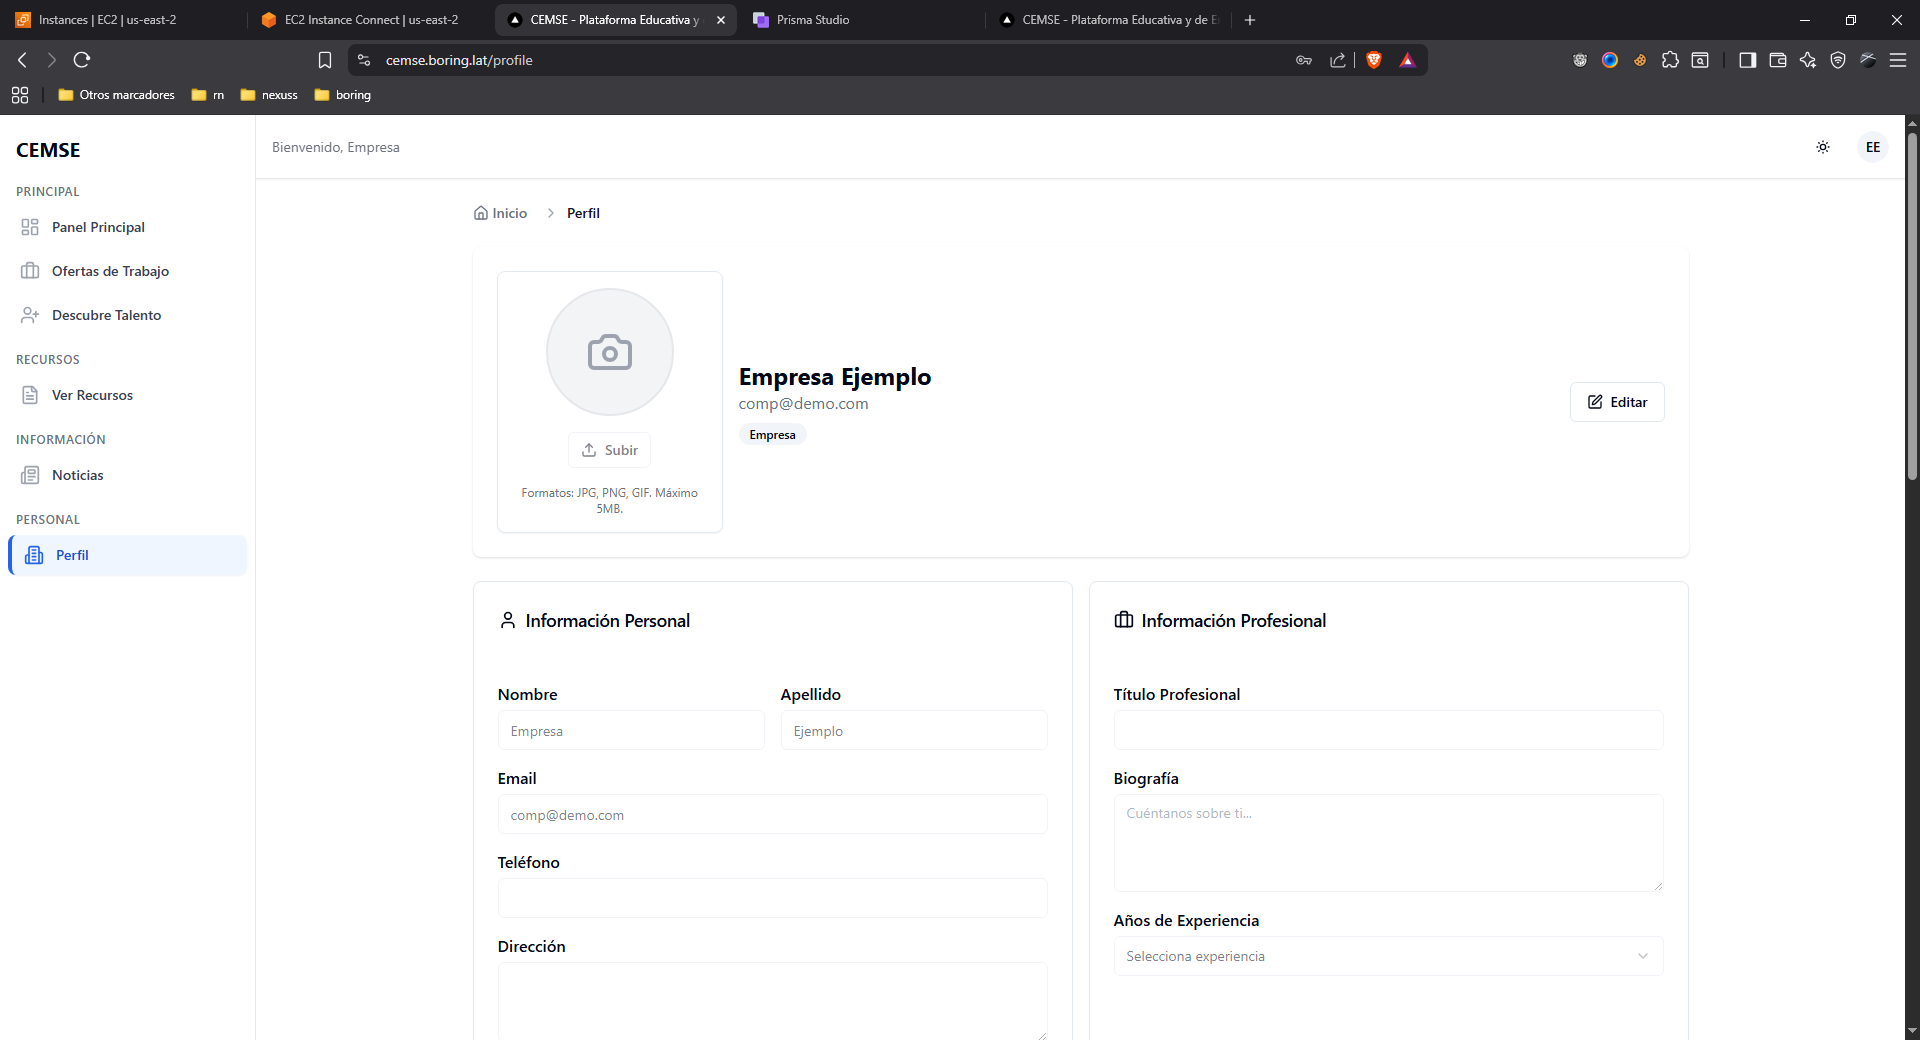
\includegraphics[width=0.9\textwidth]{screenshots/companies/profile.png}
    \caption{Perfil de la empresa}
    \label{fig:company-profile}
\end{figure}

\subsection{Flujo de Usuario Institución (INSTITUTION)}

\subsubsection{Dashboard de Institución}
\begin{figure}[H]
    \centering
    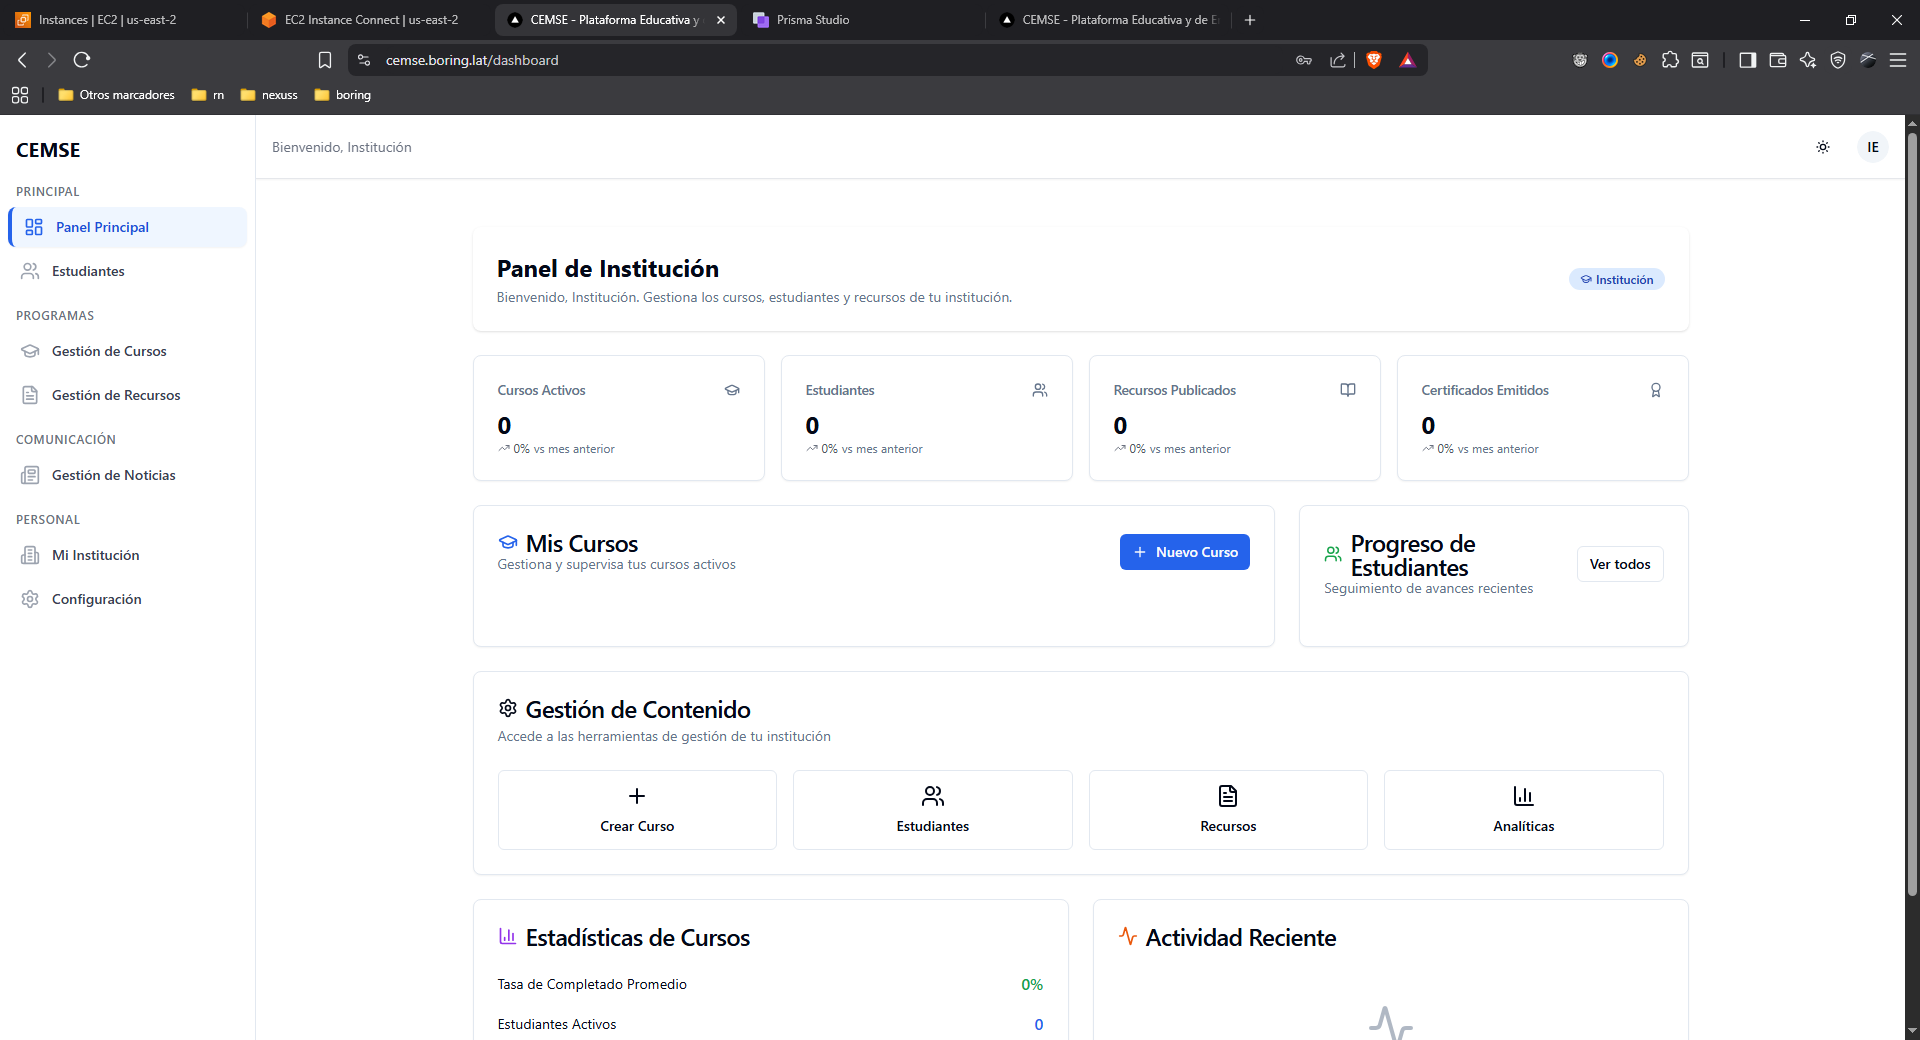
\includegraphics[width=0.9\textwidth]{screenshots/institutions/dashboard.png}
    \caption{Dashboard principal para instituciones}
    \label{fig:institution-dashboard}
\end{figure}

\subsubsection{Gestión de Usuarios (Municipio)}
\begin{figure}[H]
    \centering
    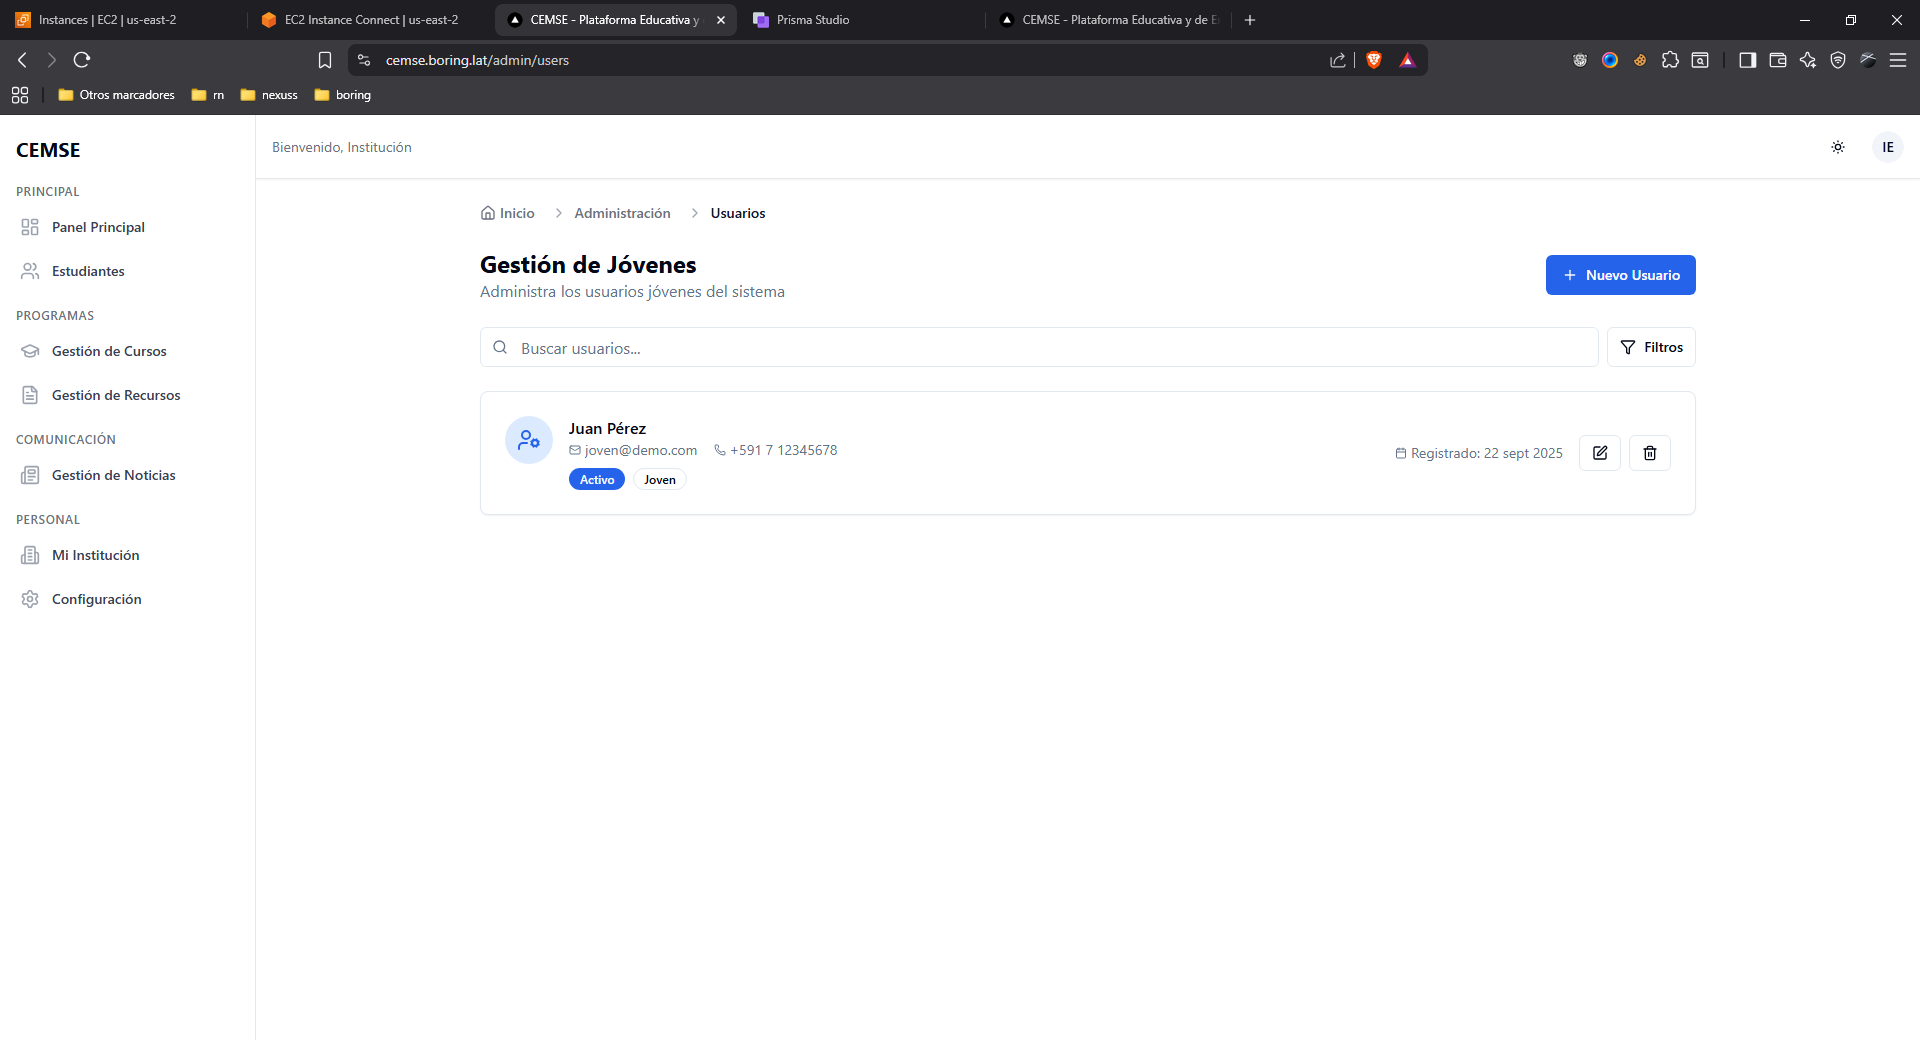
\includegraphics[width=0.9\textwidth]{screenshots/institutions/user-management.png}
    \caption{Panel de gestión de usuarios (vista municipio)}
    \label{fig:institution-users}
\end{figure}

\subsubsection{Gestión de Cursos}
\begin{figure}[H]
    \centering
    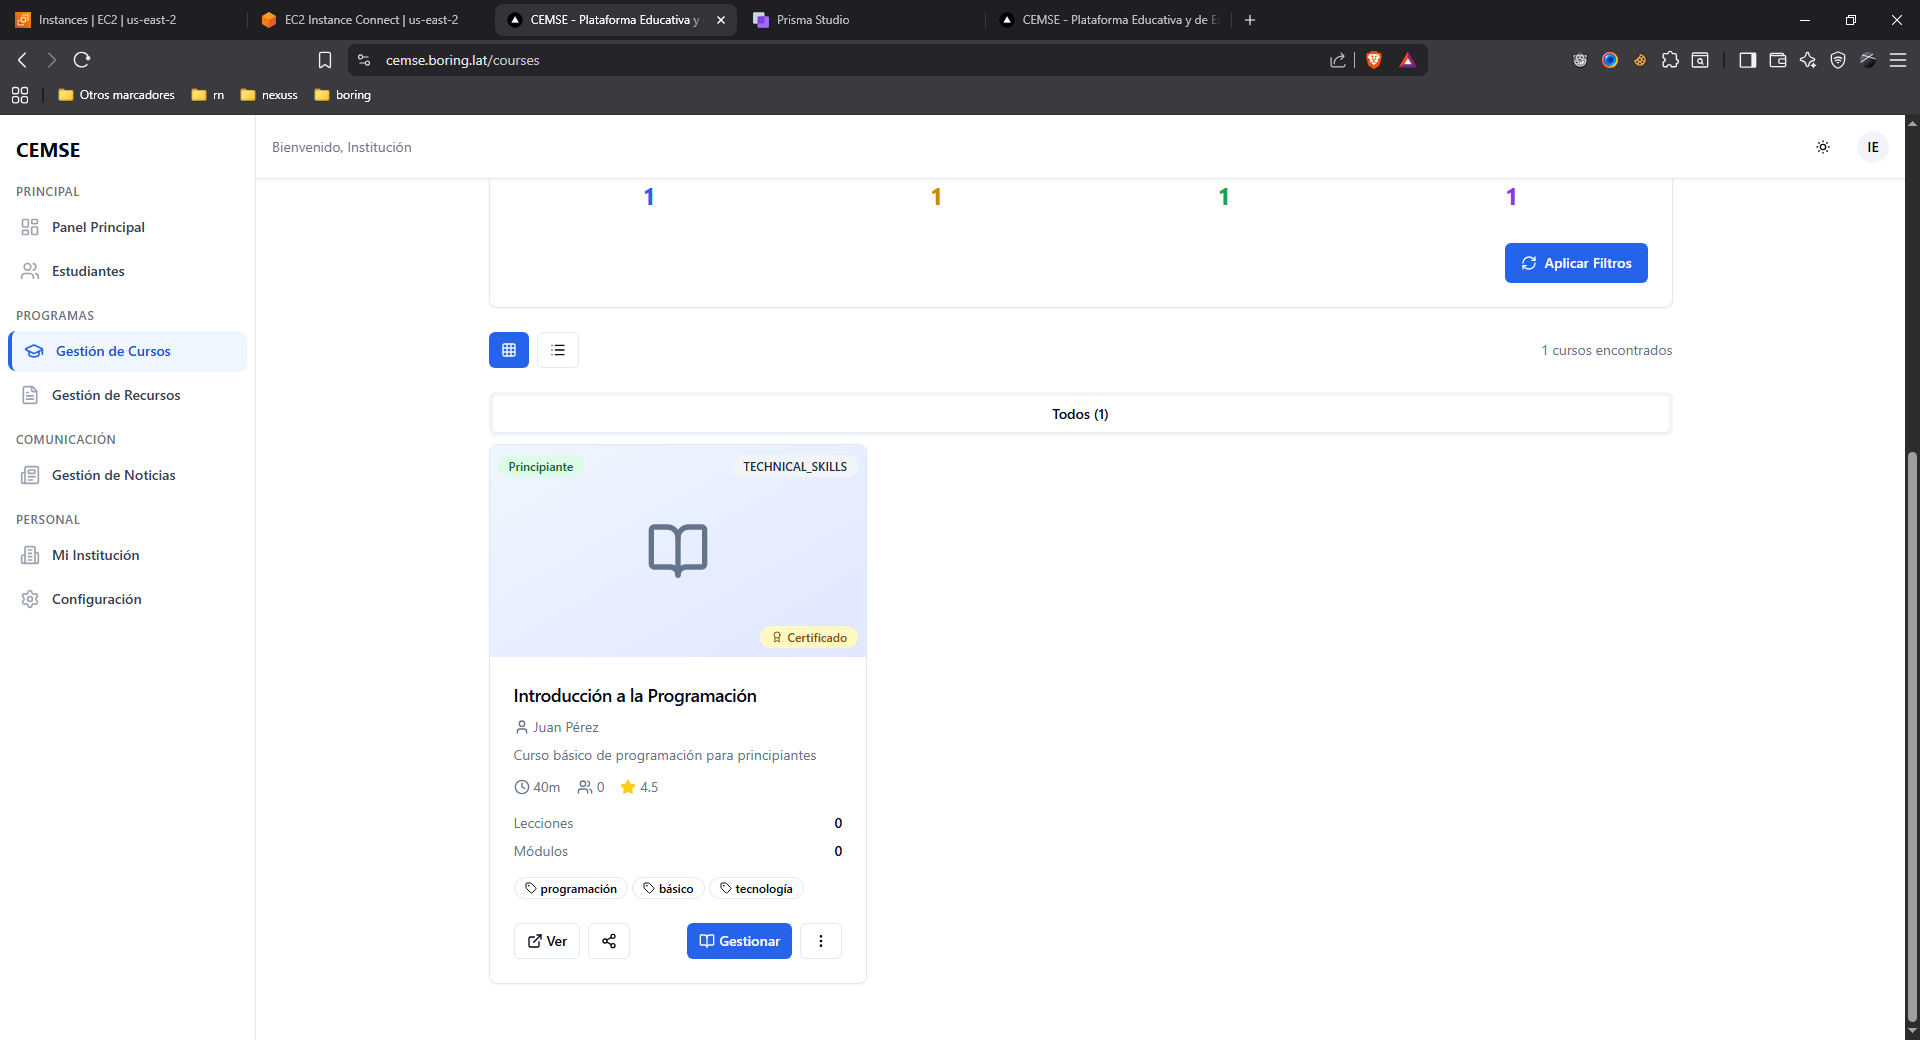
\includegraphics[width=0.9\textwidth]{screenshots/institutions/course-management.png}
    \caption{Panel de gestión de cursos}
    \label{fig:institution-courses}
\end{figure}

\subsubsection{Gestión de Estudiantes}
\begin{figure}[H]
    \centering
    \includegraphics[width=0.9\textwidth]{screenshots/institutions/student-management.png}
    \caption{Panel de gestión de estudiantes}
    \label{fig:institution-students}
\end{figure}

\subsection{Flujo de Super Administrador (SUPERADMIN)}

\subsubsection{Dashboard de Administración}
\begin{figure}[H]
    \centering
    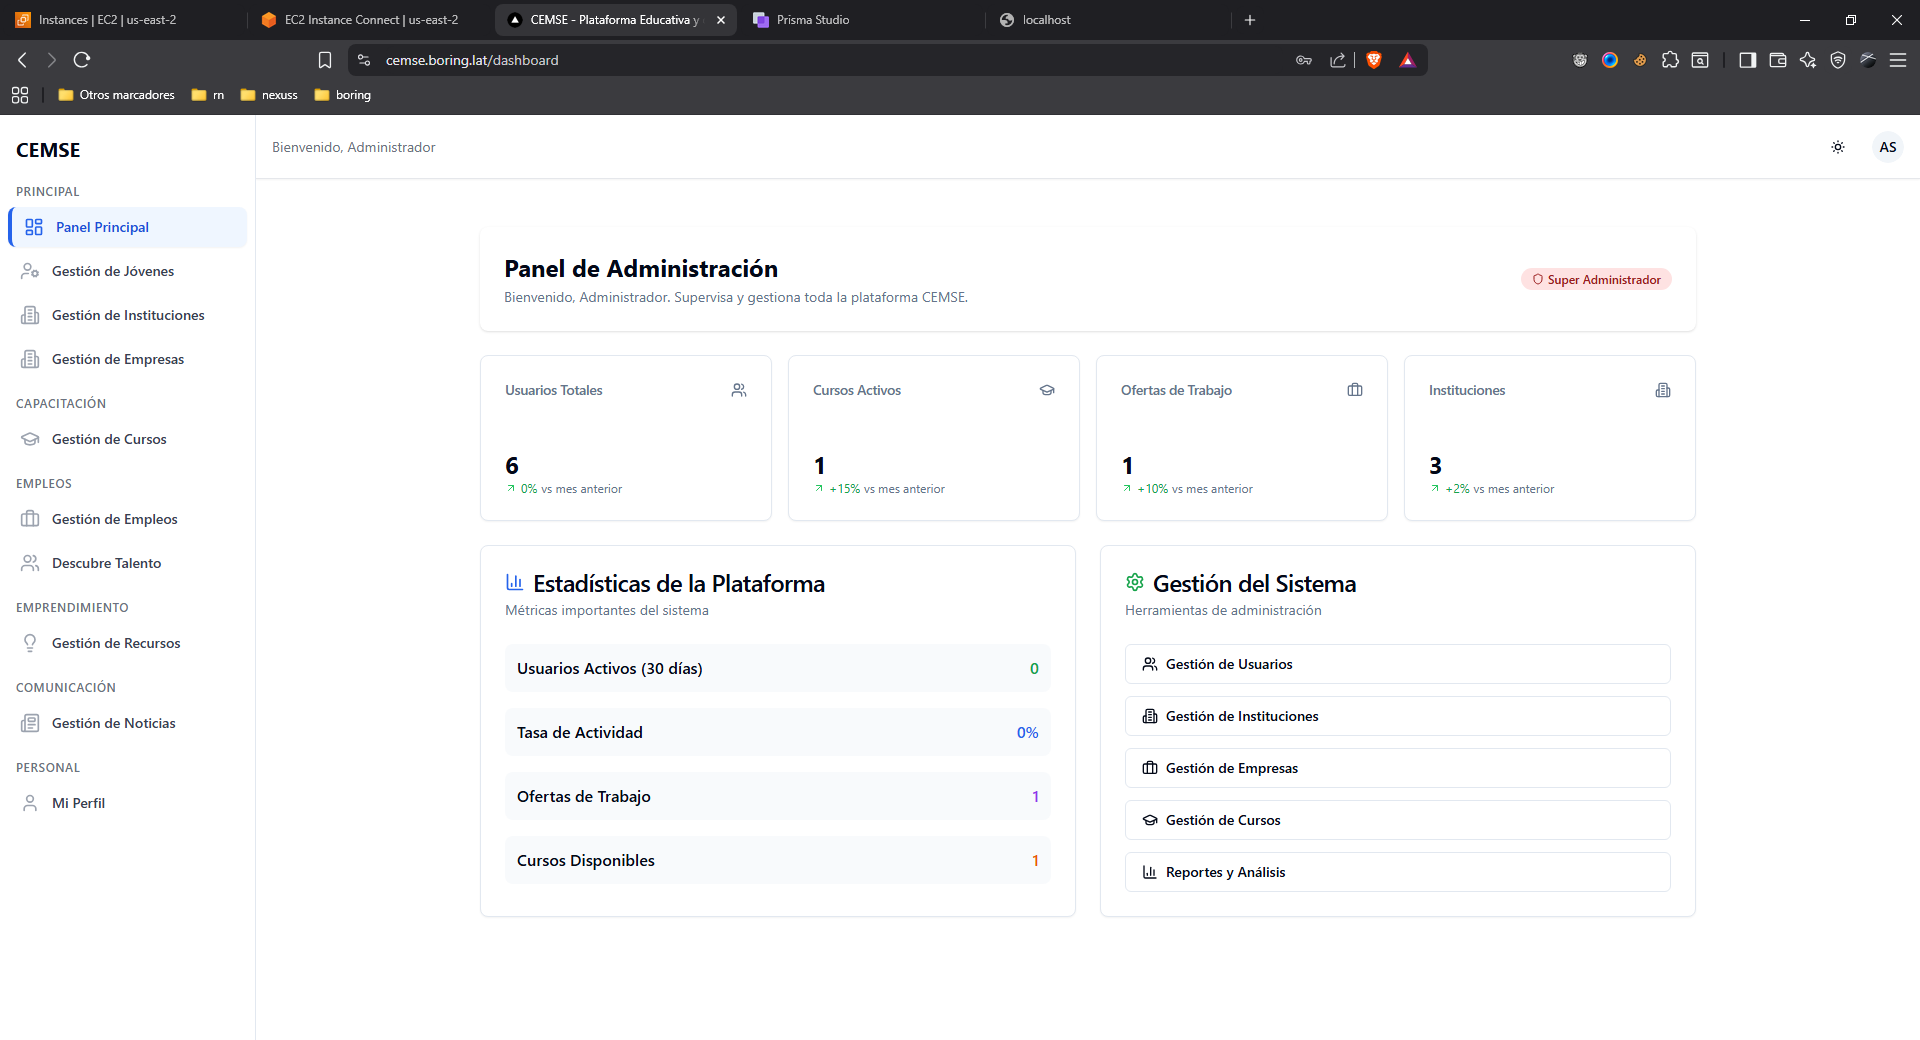
\includegraphics[width=0.9\textwidth]{screenshots/admin/dashboard.png}
    \caption{Dashboard de super administrador}
    \label{fig:admin-dashboard}
\end{figure}

\subsubsection{Gestión de Usuarios del Sistema}
\begin{figure}[H]
    \centering
    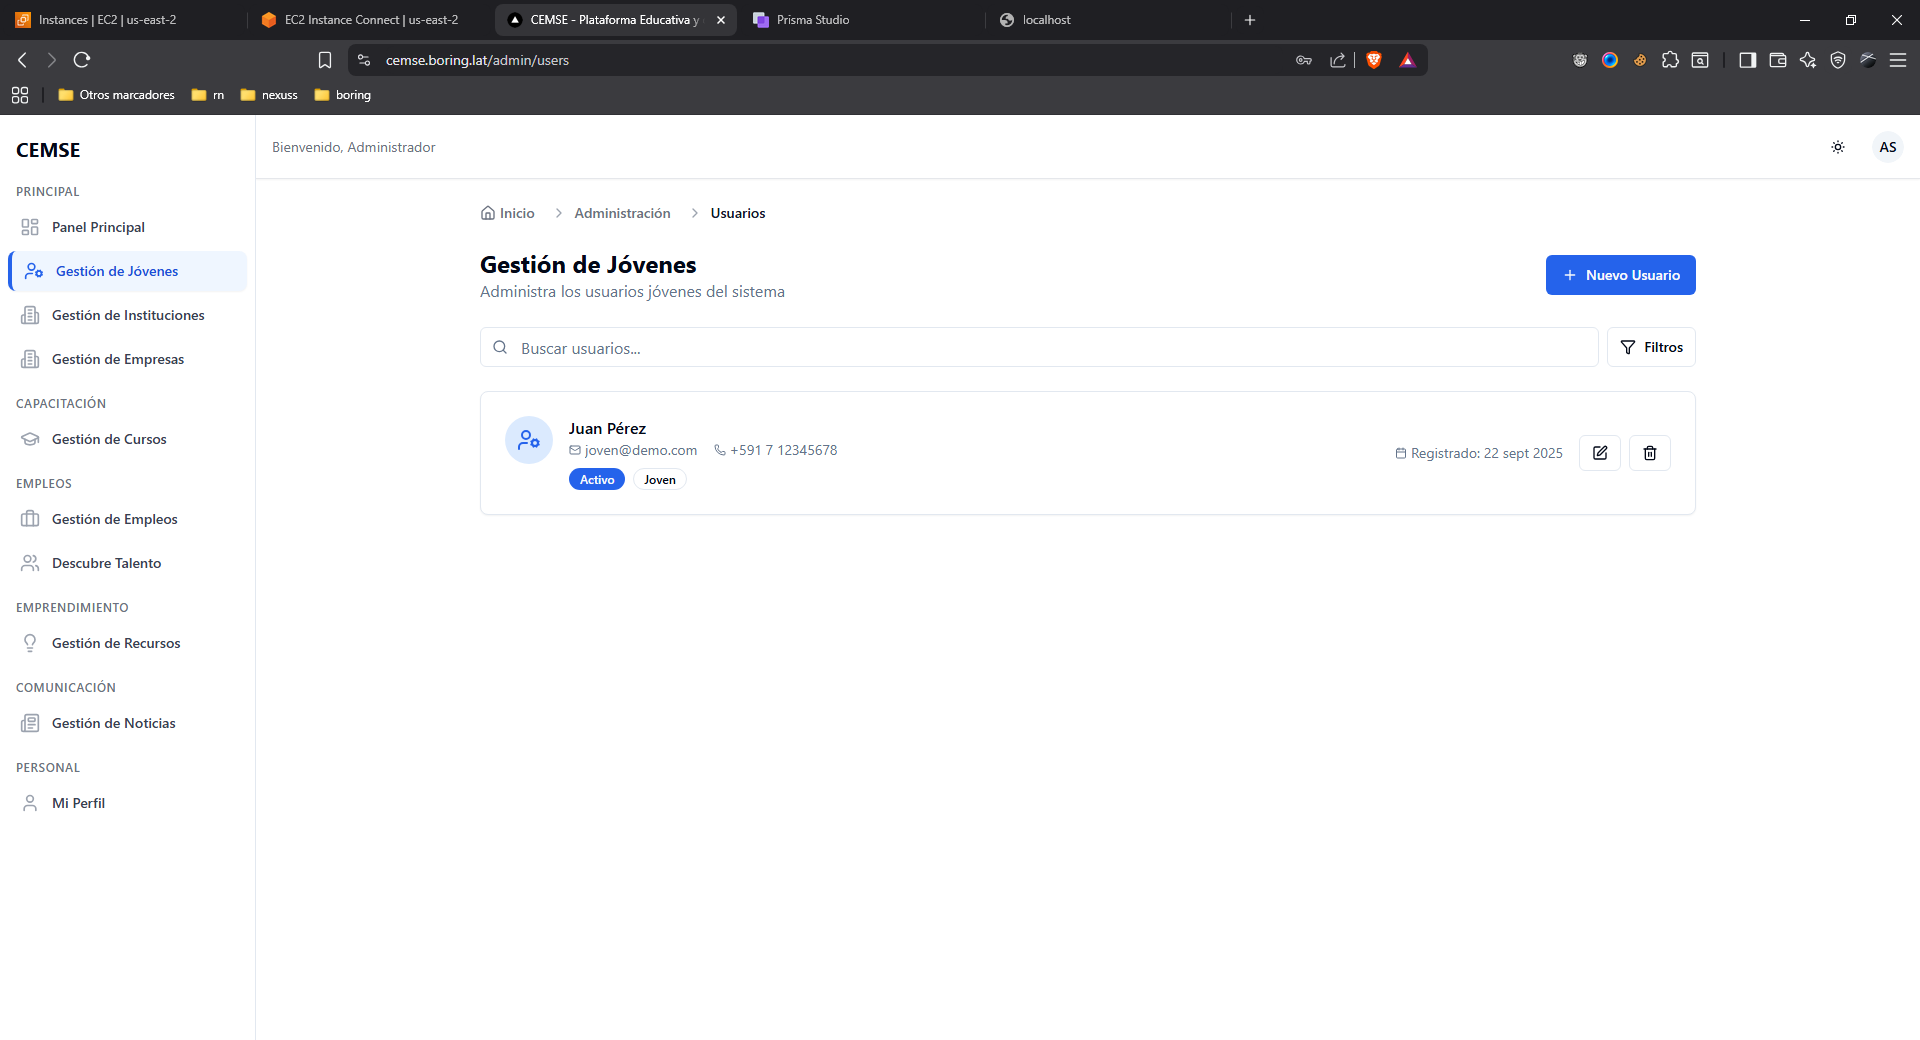
\includegraphics[width=0.9\textwidth]{screenshots/admin/user-management.png}
    \caption{Panel de gestión de usuarios del sistema}
    \label{fig:admin-users}
\end{figure}

\subsubsection{Gestión de Instituciones}
\begin{figure}[H]
    \centering
    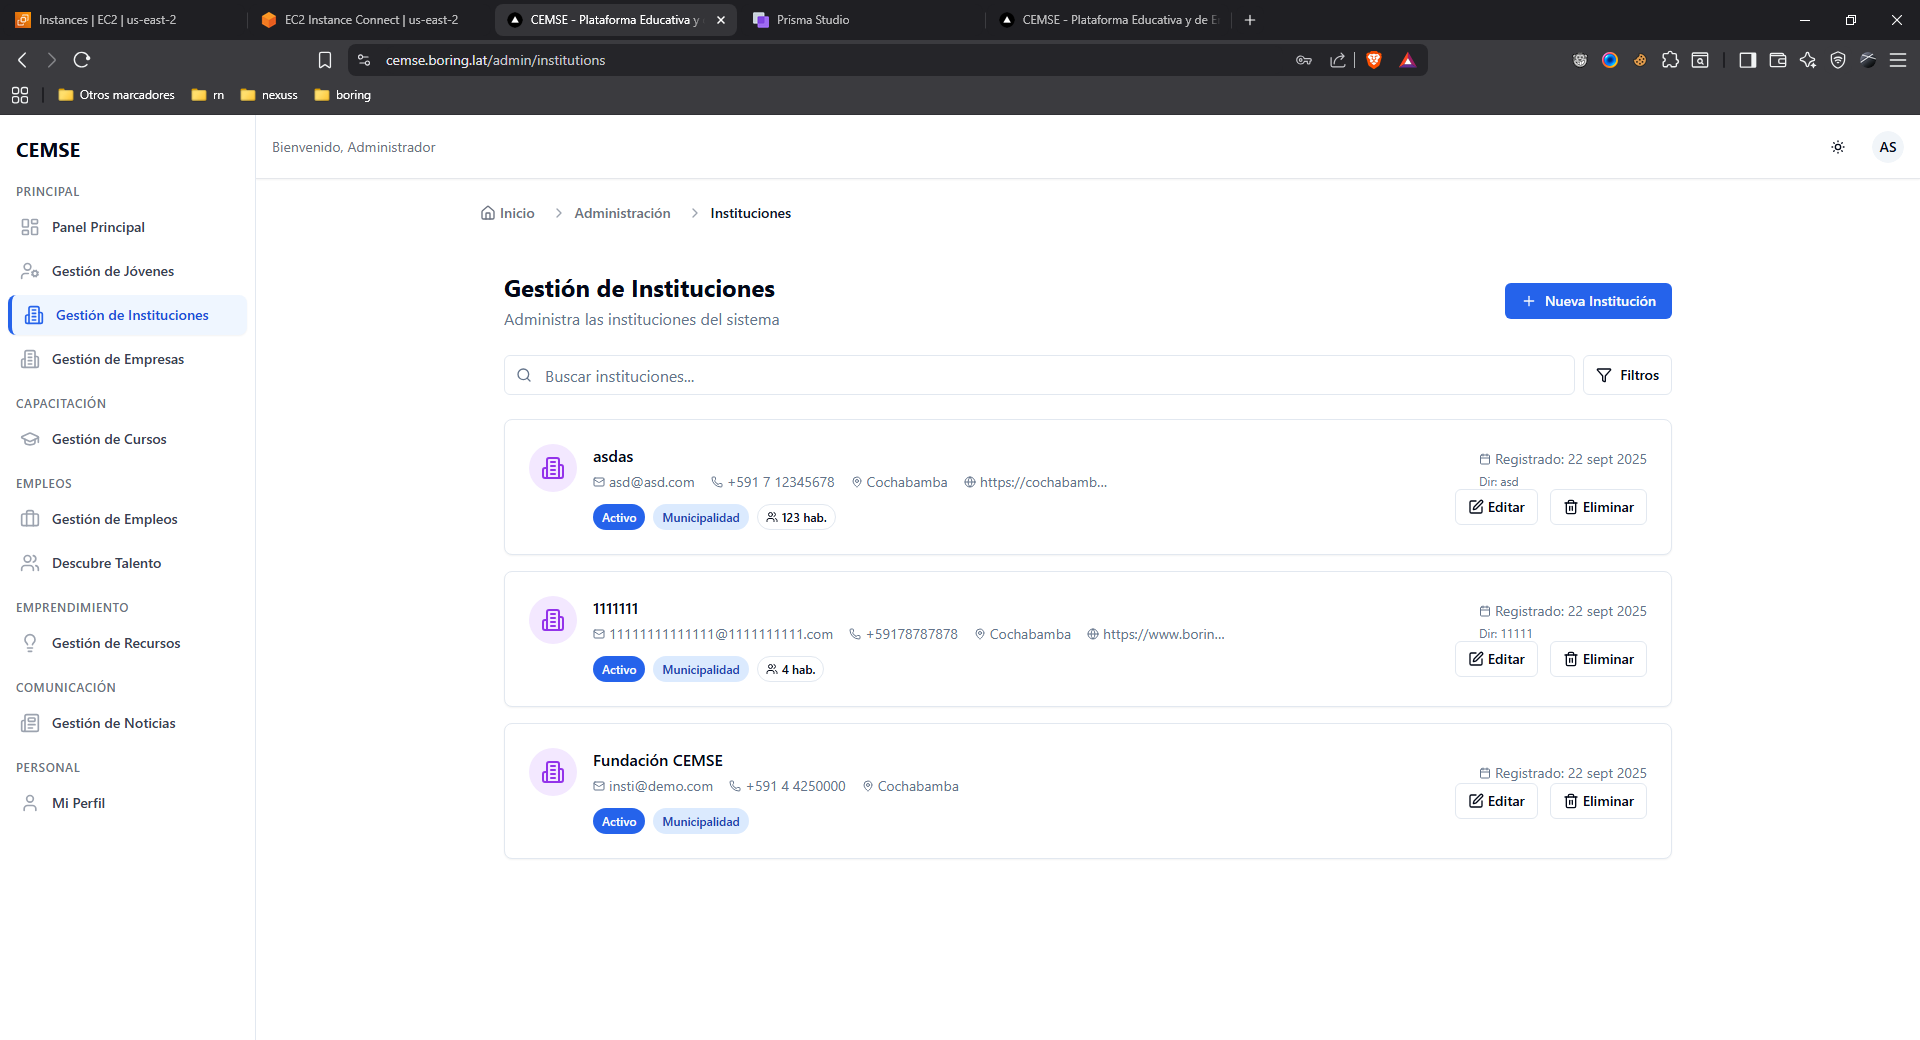
\includegraphics[width=0.9\textwidth]{screenshots/admin/institution-management.png}
    \caption{Panel de gestión de instituciones}
    \label{fig:admin-institutions}
\end{figure}

\subsubsection{Gestión de Empresas}
\begin{figure}[H]
    \centering
    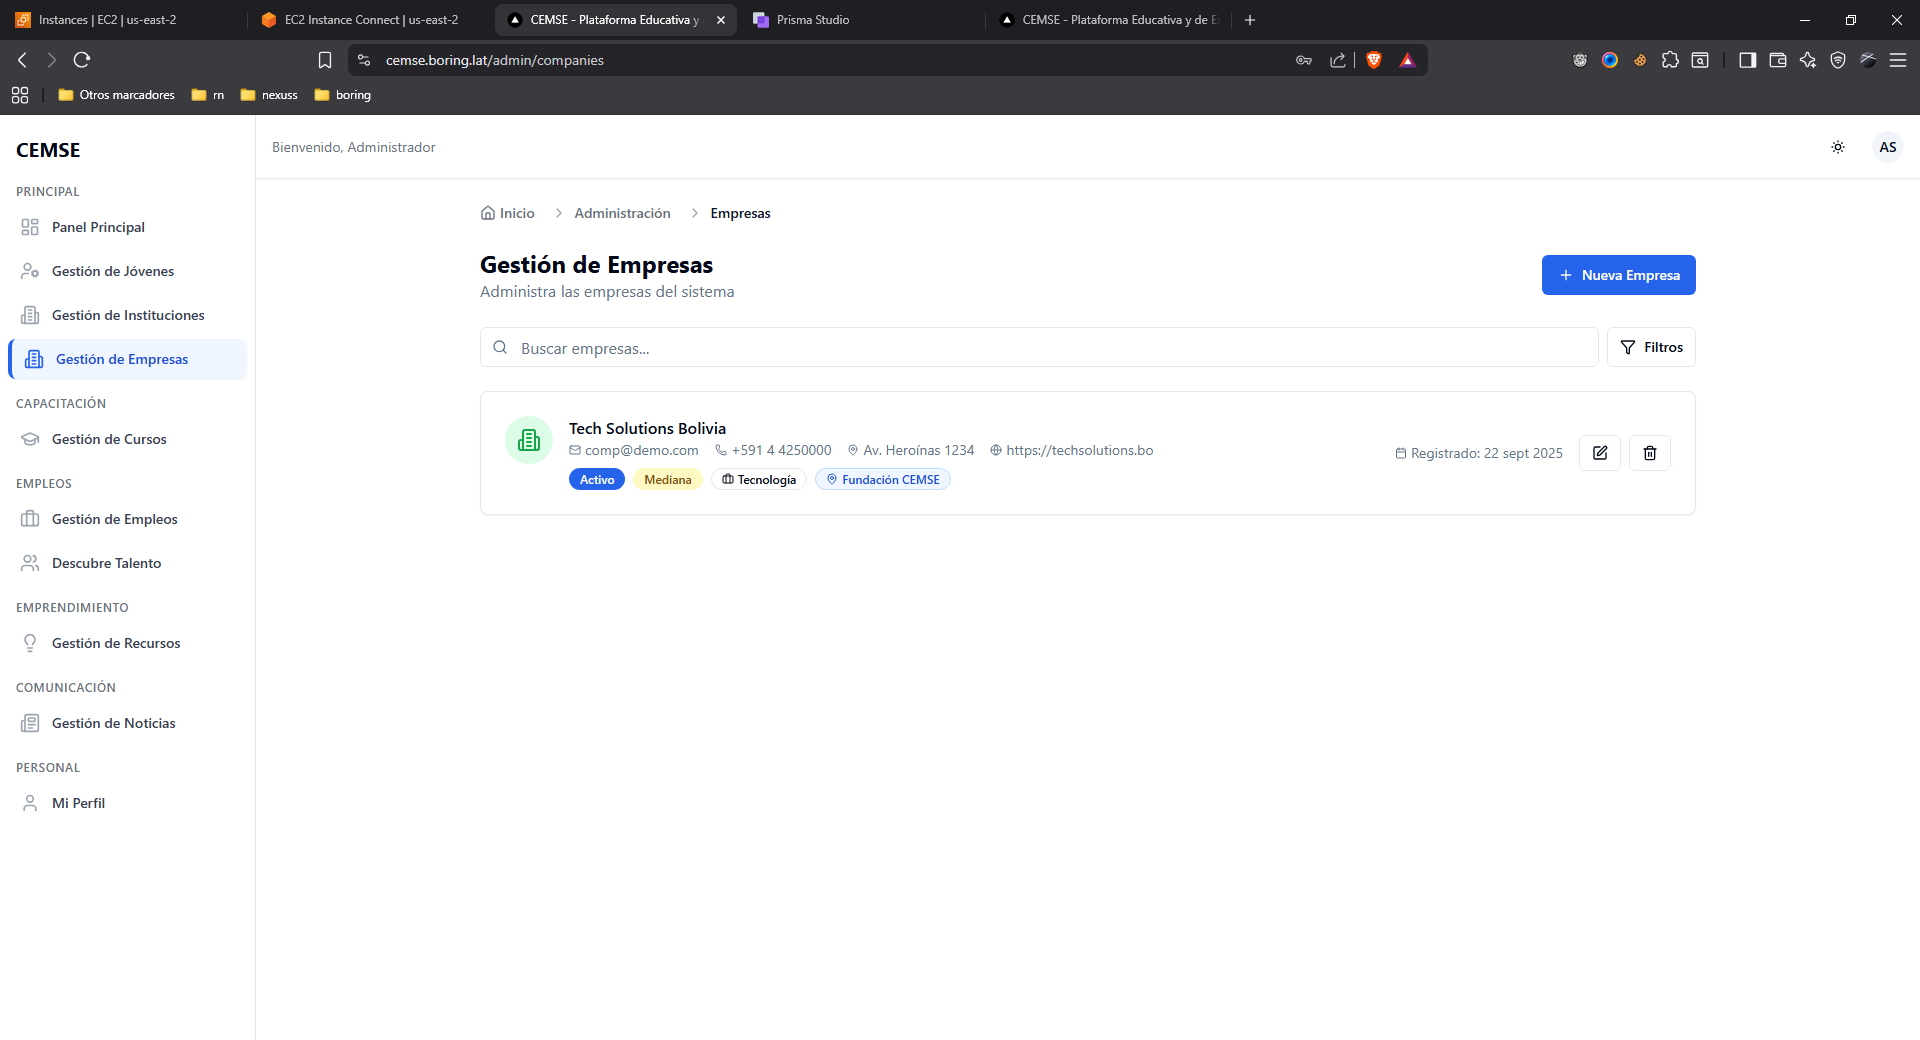
\includegraphics[width=0.9\textwidth]{screenshots/admin/company-management.png}
    \caption{Panel de gestión de empresas}
    \label{fig:admin-companies}
\end{figure}

\subsection{Características Adicionales}

\subsubsection{Sistema de Mensajería}
\begin{figure}[H]
    \centering
    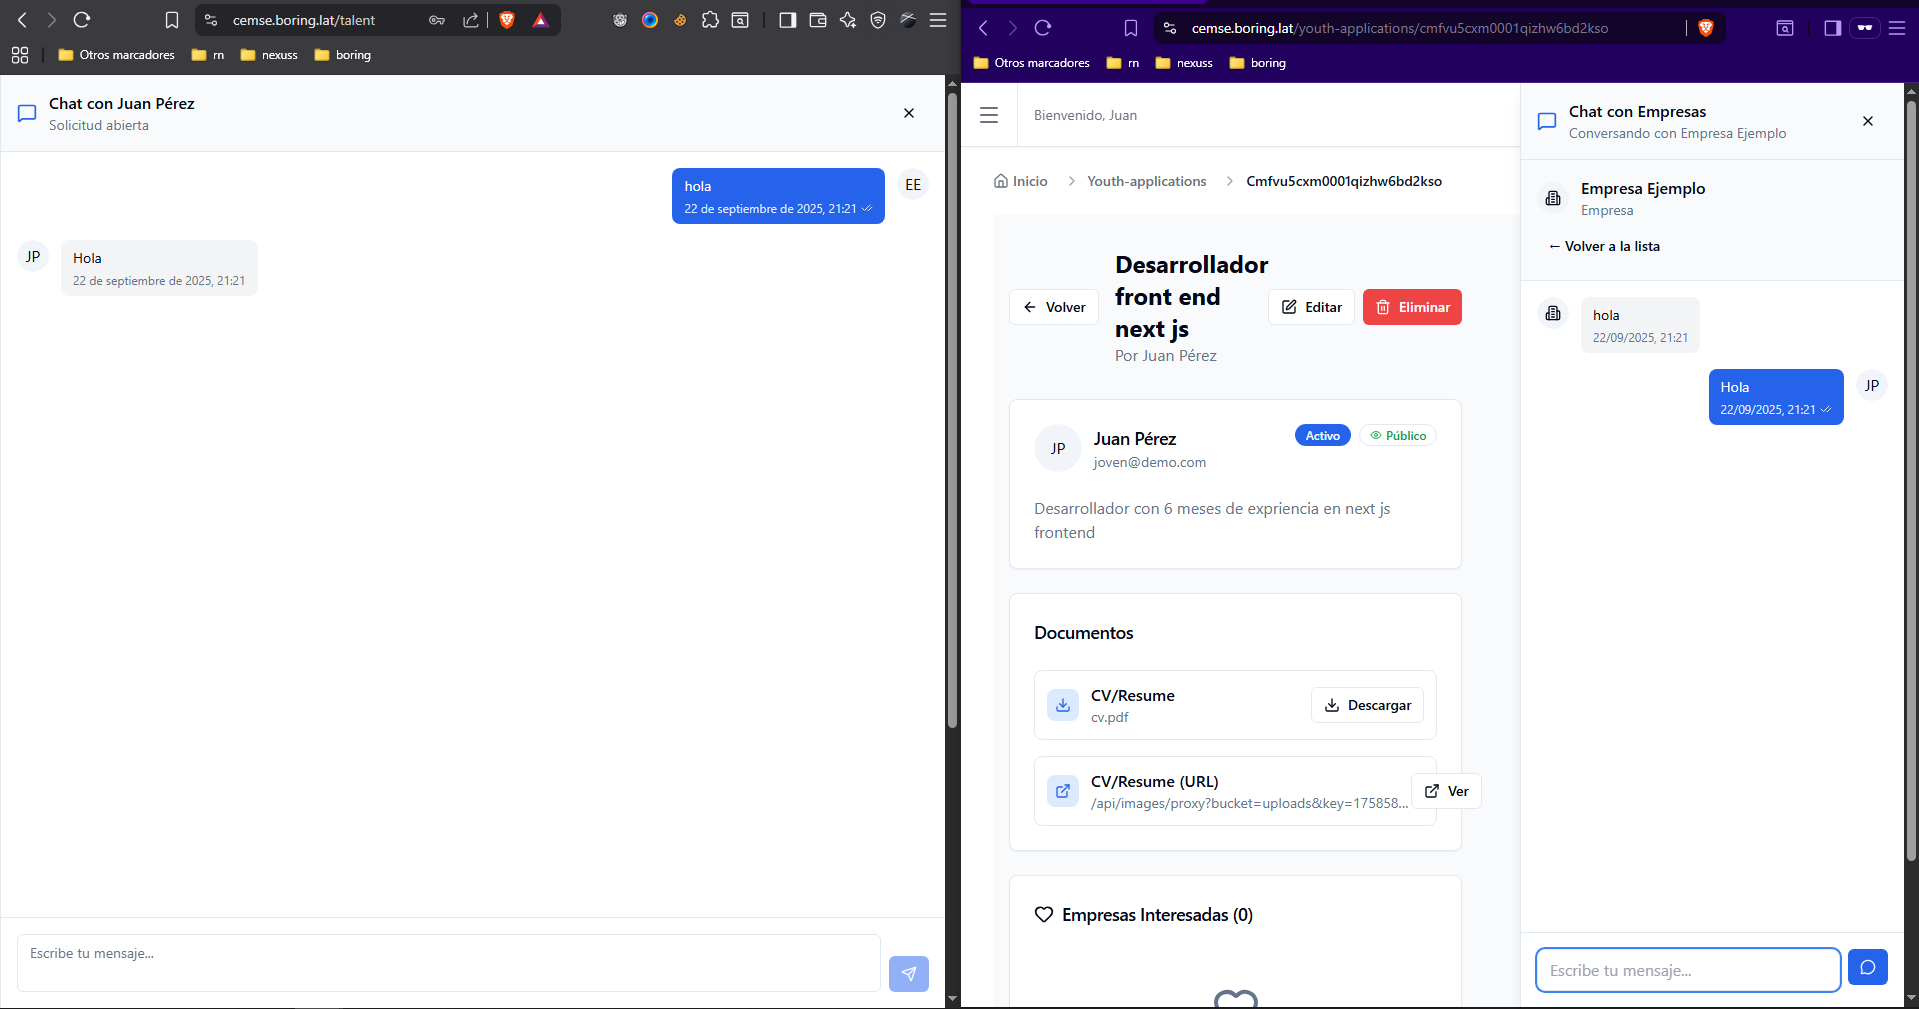
\includegraphics[width=0.9\textwidth]{screenshots/features/messaging.png}
    \caption{Sistema de mensajería integrado}
    \label{fig:messaging}
\end{figure}

\subsubsection{Portal de Noticias}
\begin{figure}[H]
    \centering
    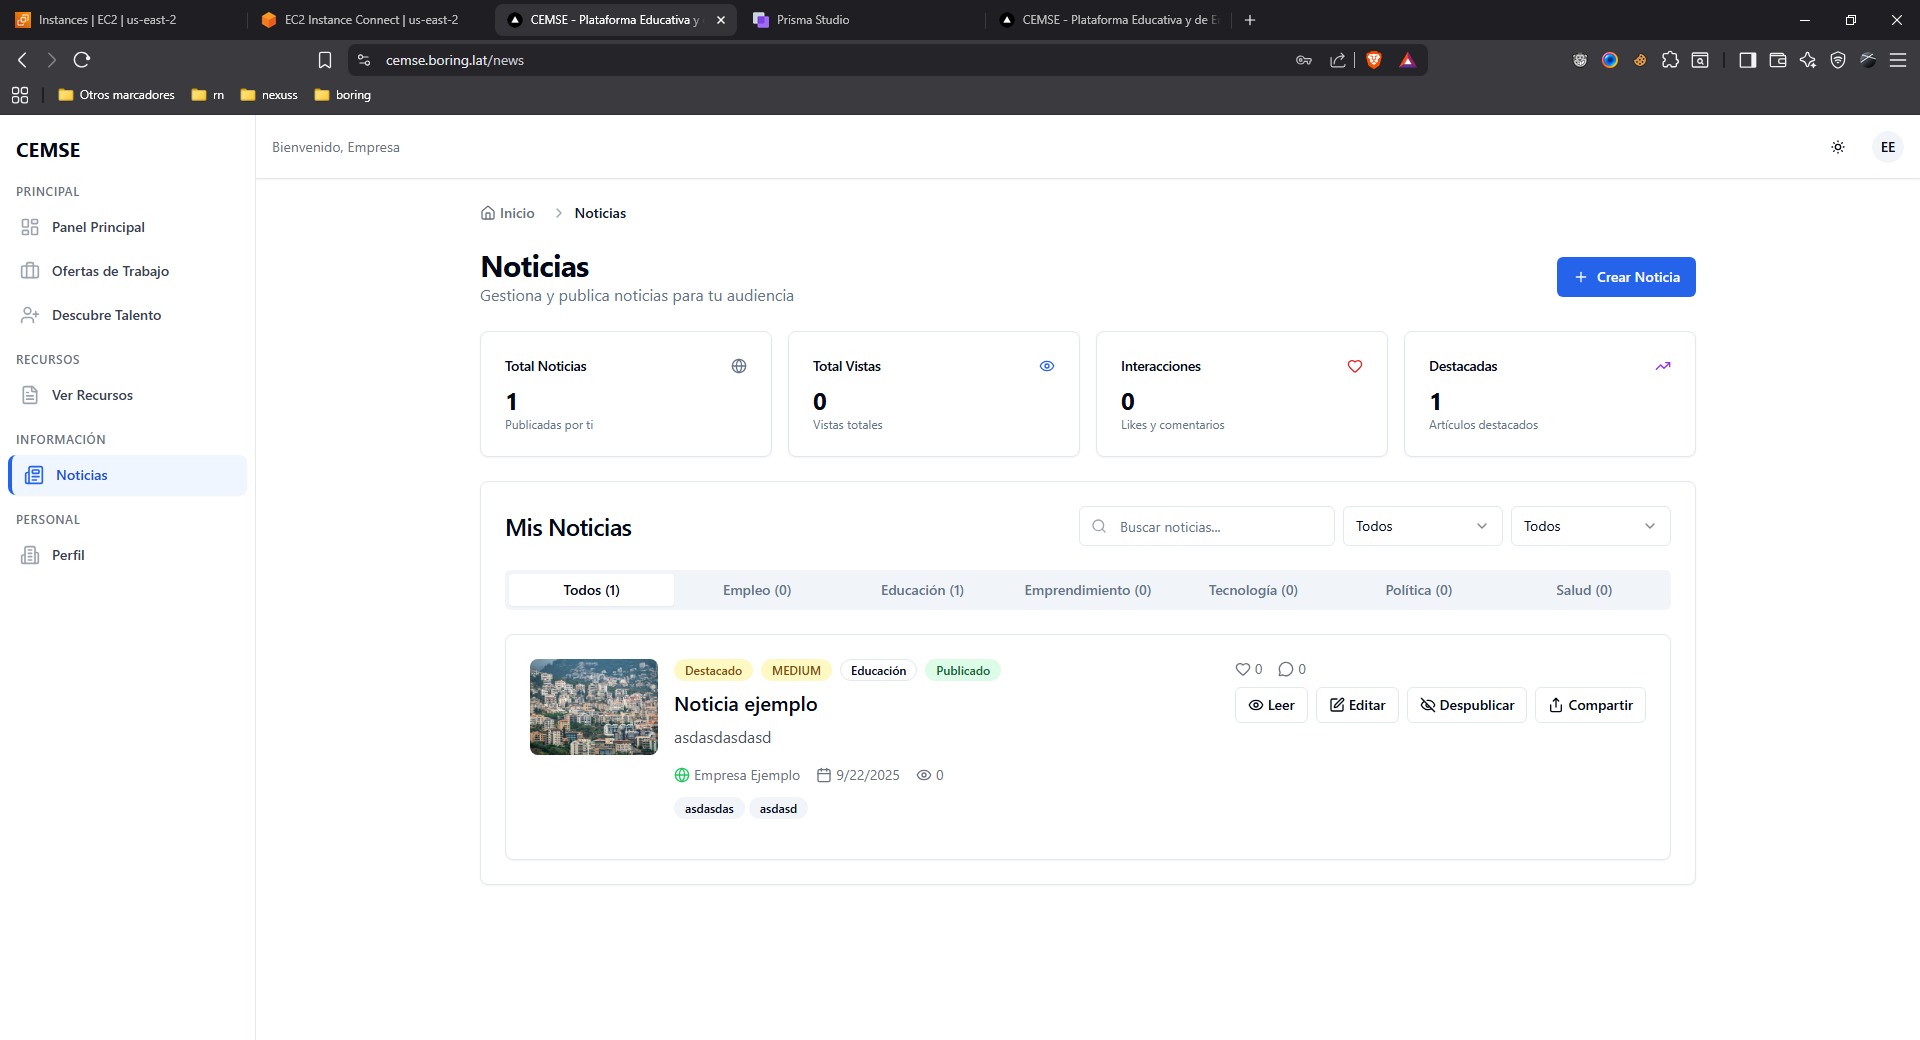
\includegraphics[width=0.9\textwidth]{screenshots/features/news.png}
    \caption{Portal de noticias y comunicaciones}
    \label{fig:news}
\end{figure}

\subsubsection{Recursos Educativos}
\begin{figure}[H]
    \centering
    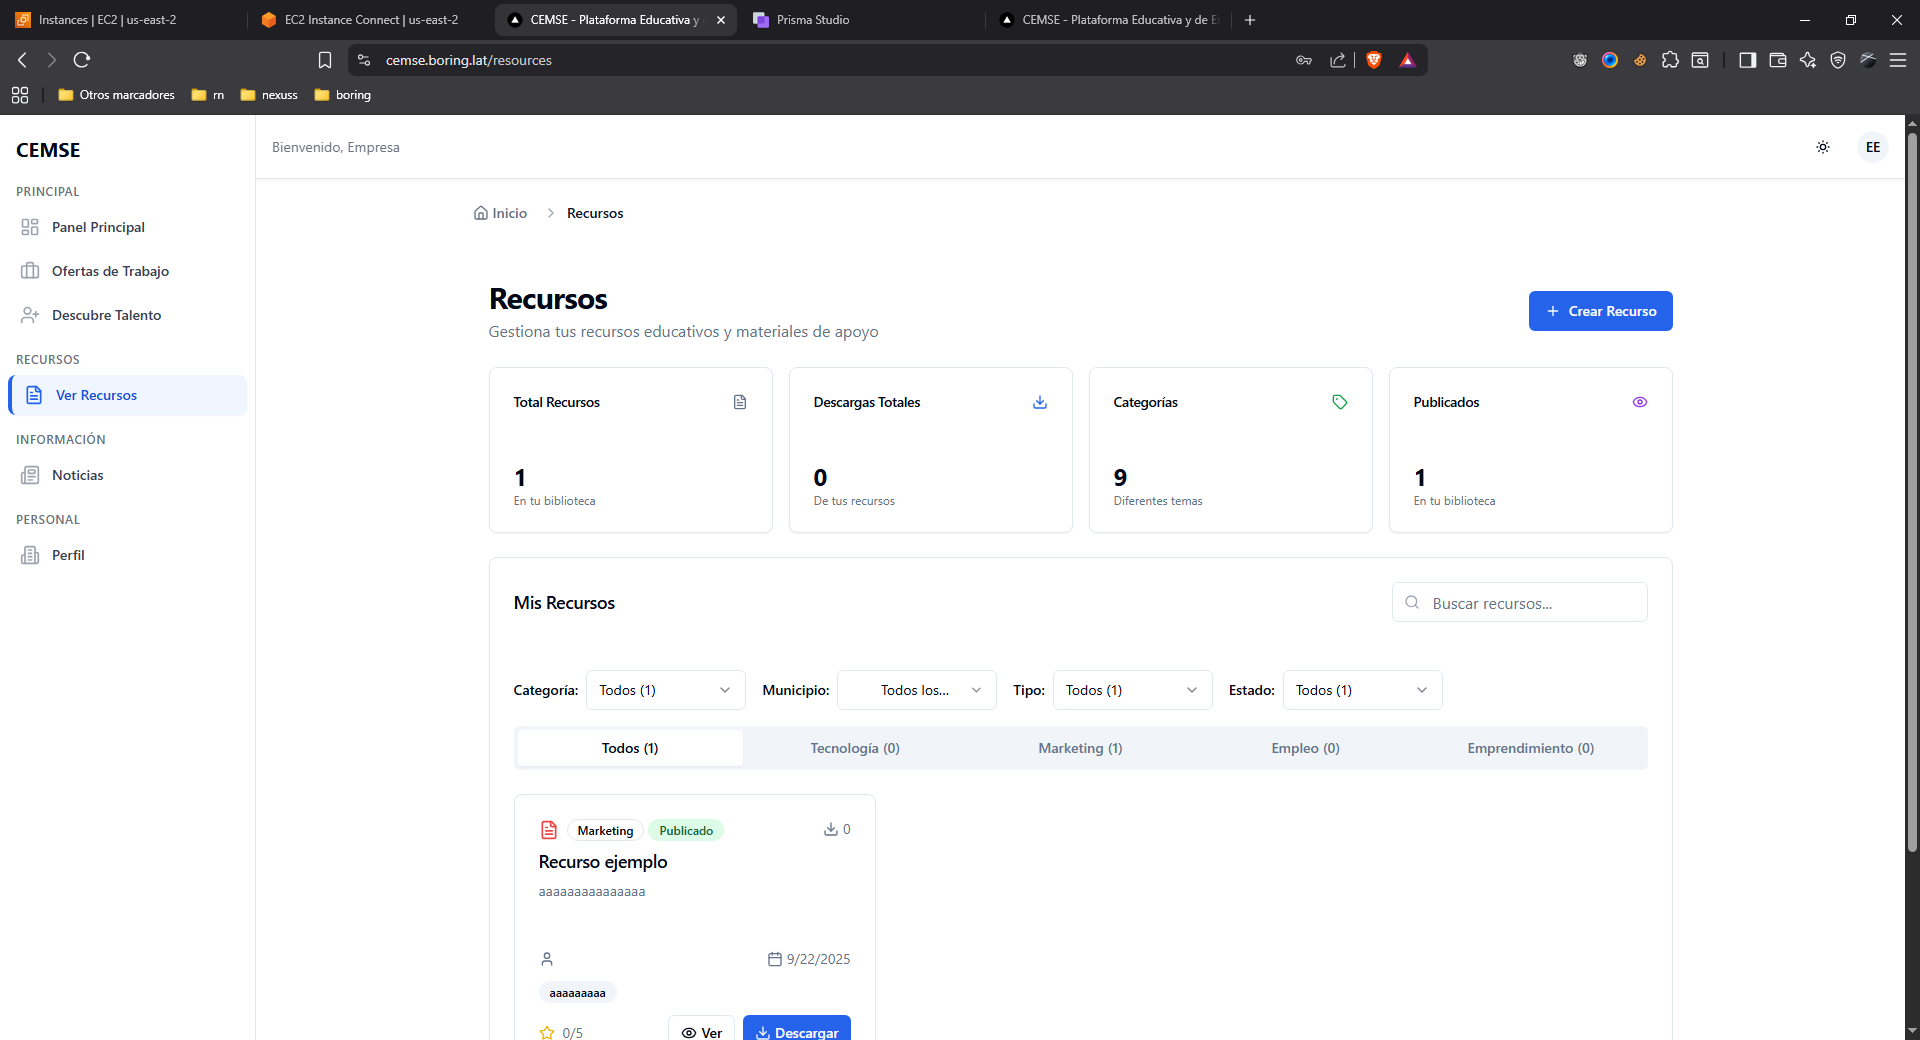
\includegraphics[width=0.9\textwidth]{screenshots/features/resources.png}
    \caption{Portal de recursos educativos}
    \label{fig:resources}
\end{figure}

\subsection{Conclusión del Tour Visual}

Este tour visual demuestra la amplitud y profundidad de la plataforma CEMSE, mostrando interfaces intuitivas y funcionalidades especializadas para cada tipo de usuario. La plataforma integra de manera cohesiva la gestión educativa, el empleo juvenil y el emprendimiento en un ecosistema digital completo.

Las capturas de pantalla evidencian:
\begin{itemize}
    \item \textbf{Interfaz moderna:} Diseño responsive con Tailwind CSS
    \item \textbf{Navegación intuitiva:} Sidebar contextual por rol de usuario
    \item \textbf{Funcionalidades especializadas:} Herramientas específicas para cada actor
    \item \textbf{Integración completa:} Flujos conectados entre módulos
    \item \textbf{Experiencia de usuario:} Interfaces limpias y funcionales
\end{itemize}

\end{document}